
% ----------------------------------------------------------------------
%                   LATEX TEMPLATE FOR PhD THESIS
% ----------------------------------------------------------------------

% based on Harish Bhanderi's PhD/MPhil template, then Uni Cambridge
% http://www-h.eng.cam.ac.uk/help/tpl/textprocessing/ThesisStyle/
% corrected and extended in 2007 by Jakob Suckale, then MPI-CBG PhD programme
% and made available through OpenWetWare.org - the free biology wiki


%: Style file for Latex
% Most style definitions are in the external file PhDthesisPSnPDF.
% In this template package, it can be found in ./Latex/Classes/
\documentclass[twoside,12pt]{Latex/Classes/PhDthesisPSnPDF}

\makeatletter
        \setlength{\@fptop}{0pt}
\makeatother


%: Macro file for Latex
% Macros help you summarise frequently repeated Latex commands.
% Here, they are placed in an external file /Latex/Macros/MacroFile1.tex
% An macro that you may use frequently is the figuremacro (see introduction.tex)
\include{Latex/Macros/MacroFile1}
\usepackage[table]{xcolor}
%% The amssymb package provides various useful mathematical symbols
\usepackage{amssymb}

%% The amsthm package provides extended theorem environments
\usepackage{amsthm}

%% amsmath for math environment
\usepackage{amsmath}

\DeclareMathOperator*{\argmin}{arg\,min}
\DeclareMathOperator*{\argmax}{arg\,max}
\DeclareMathOperator*{\sign}{sign}
\DeclareMathOperator*{\infspie}{inf}


% to break equation
%\usepackage{mathpazo}
%\usepackage{mathptmx}
%\usepackage[mathpazo]{flexisym}
%\usepackage{breqn}

%% For clever reference
%\usepackage{cleveref}

%% color package
\usepackage{color}

%% figure package
\usepackage{epsf,graphicx}
\usepackage{epstopdf}
\usepackage{subfigure}	
\usepackage{transparent}

%% New environment to have some indent inside enumerate environment
\usepackage{enumitem}

%% To create acronym for proper glossary
\usepackage{acro}

%% To number the line in the article
\usepackage{lineno}

%% Environment to include table with notes
\usepackage{array}
\usepackage{threeparttable}
\usepackage{booktabs}
\usepackage{multirow}
\usepackage{siunitx}

%% In order to change size of margin
\usepackage{geometry}
\usepackage{changepage}
\usepackage{lscape}
%% Colorpackage for table
\usepackage{colortbl}
\usepackage{tabularx}
\usepackage{arydshln}

%% To use URL referencing
\usepackage{url}
%\usepackage[hidelinks]{hyperref}

%% In order to draw some graphs
\usepackage{tikz,xifthen}
\usepackage{tikz-qtree}
\usetikzlibrary{decorations.pathmorphing} % noisy shapes
\usetikzlibrary{fit}					% fitting shapes to coordinates
\usetikzlibrary{backgrounds}	% drawing the background after the foreground
\usetikzlibrary{shapes,arrows,shadows}
\usetikzlibrary{calc,decorations.pathreplacing,decorations.markings,positioning}
\usetikzlibrary{snakes,decorations.text,shapes,patterns}
%\usepackage{scalefnt,lmodern,booktabs}

%% Paxkage for cross and tick symbols
\usepackage{pifont}
\newcommand{\cmark}{\color{green!60!black!80}\ding{51}}
\newcommand{\mmark}{{\color{green!60!black!80}\ding{51}}$^{!}$}
\newcommand{\xmark}{\color{red!60!black!80}\ding{55}}
\newcommand{\cmarksmall}{\color{green!60!black!80}\ding{51}}
\newcommand{\mmarksmall}{{\color{green!60!black!80}\ding{51}}$^{!}$}
\newcommand{\xmarksmall}{\color{red!60!black!80}\ding{55}}
\newcommand{\Conv}{\mathop{\scalebox{1.5}{\raisebox{-0.2ex}{$\ast$}}}}%

\definecolor{autoGuided}{rgb}{ 0.3765    0.7294    0.9412}
\newcommand{\autoGuidedColor}{(light-Blue)}
\definecolor{fullyAuto}{rgb}{ 0.0941    0.3843    0.6627}
\newcommand{\fullyAutoColor}{(dark-blue)}
\definecolor{semiAuto}{rgb}{ 0.0784    0.5059    0.1686}
\newcommand{\semiAutoColor}{(light-green)}
\definecolor{fullyGuided}{rgb}{ 0.4275    0.6902    0.3176}
\newcommand{\fullyGuidedColor}{(dark-green)}

\DeclareSIUnit\ppm{ppm}
\DeclareSIUnit\px{px}

\usepackage{ltxtable}
\usepackage{listings}
\usepackage{color}
\usepackage[toc]{appendix}
 
\definecolor{codegreen}{rgb}{0,0.6,0}
\definecolor{codegray}{rgb}{0.5,0.5,0.5}
\definecolor{codepurple}{rgb}{0.58,0,0.82}
\definecolor{backcolour}{rgb}{0.95,0.95,0.92}
 
\lstdefinestyle{mystyle}{
    backgroundcolor=\color{backcolour},   
    commentstyle=\color{codegreen},
    keywordstyle=\color{magenta},
    numberstyle=\tiny\color{codegray},
    stringstyle=\color{codepurple},
    basicstyle=\footnotesize,
    breakatwhitespace=false,         
    breaklines=true,                 
    captionpos=b,                    
    keepspaces=true,                 
    numbers=left,                    
    numbersep=5pt,                  
    showspaces=false,                
    showstringspaces=false,
    showtabs=false,                  
    tabsize=2
}
 
\lstset{style=mystyle}
%\acrodef{cap}[CaP]{prostate cancer}
\DeclareAcronym{cap}{
short = CaP,
long = prostate cancer
}
%\acrodef{cade}[CADe]{computer-aided detection}
\DeclareAcronym{cade}{
short = CADe,
long = computer-aided detection
}
%\acrodef{cadx}[CADx]{computer-aided diagnosis}
\DeclareAcronym{cadx}{
short = CADx,
long = computer-aided diagnosis
}
\DeclareAcronym{lm}{
short = LM, 
long = Leung-Malik set
}
%\acrodef{us}[US]{ultrasound}
\DeclareAcronym{us}{
short = US,
long = ultrasound
}
%\acrodef{ct}[CT]{computer tomography}
\DeclareAcronym{ct}{
short = CT,
long = computer tomography
}
%\acrodef{cad}[CAD]{computer-aided detection and diagnosis}
\DeclareAcronym{cad}{
short = CAD,
long = computer-aided detection and diangosis
}
%\acrodef{mri}[MRI]{magnetic resonance imaging}
\DeclareAcronym{mri}{
short = MRI,
long = magnetic resonance imaging
}
%\acrodef{nmr}[NMR]{nuclear magnetic resonance}
\DeclareAcronym{nmr}{
short = NMR,
long = nuclear magnetic resonance
}

\DeclareAcronym{omp}{
  short = OMP,
  long =  Orthogonal Matching Pursuit 
}
\DeclareAcronym{adb}{
  short = AdB, 
  long = AdaBoost
}
\DeclareAcronym{gb}{
  short = GB, 
  long = Gradient Boosting
}

\DeclareAcronym{mp}{
  short = MP,
  long =  Matching Pursuit 
}
%\acrodef{t2w}[T$_2$-W]{T$_2$ Weighted}
\DeclareAcronym{t2w}{
short = T$_2$-W,
long = T$_2$ Weighted
}
%\acrodef{dce}[DCE]{dynamic contrast-enhanced}
\DeclareAcronym{dce}{
short = DCE,
long = dynamic contrast-enhanced
}
%\acrodef{dw}[DW]{diffusion weighted}
\DeclareAcronym{dw}{
short = DW,
long = diffusion weighted
}
%\acrodef{mrsi}[MRSI]{magnetic resonance spectroscopy imaging}
\DeclareAcronym{mrsi}{
short = MRSI,
long = magnetic resonance spectroscopy imaging
}
%\acrodef{bph}[BPH]{benign prostatic hyperplasia}
\DeclareAcronym{bph}{
short = BPH,
long = benign prostatic hyperplasia
}
%\acrodef{pz}[PZ]{peripheral zone}
\DeclareAcronym{pz}{
short = PZ,
long = peripheral zone
}
%\acrodef{cz}[CZ]{central zone}

\DeclareAcronym{mpmri}{
short = mp-MRI,
long = multiparametric \ac{mri}
}
\DeclareAcronym{cz}{
short = CZ,
long = central zone
}
%\acrodef{tz}[TZ]{transitional zone}
\DeclareAcronym{tz}{
short = TZ,
long = transitional zone
}
%\acrodef{cg}[CG]{central gland}
\DeclareAcronym{cg}{
short = CG,
long = central gland
}
%\acrodef{psa}[PSA]{prostate-specific antigen}
\DeclareAcronym{psa}{
short = PSA,
long = prostate-specific antigen
}
%\acrodef{trus}[TRUS]{transrectal ultrasound}
\DeclareAcronym{trus}{
short = TRUS,
long = transrectal ultrasound
}
%\acrodef{tr}[TR]{repetition time}
\DeclareAcronym{tr}{
short = TR,
long = repetition time
}
%\acrodef{te}[TE]{echo time}
\DeclareAcronym{te}{
short = TE,
long = echo time
}
%\acrodef{si}[SI]{signal intensity}
\DeclareAcronym{si}{
short = SI,
long = signal intensity
}
%\acrodef{ees}[EES]{extravascular-extracellular space}
\DeclareAcronym{ees}{
short = EES,
long = extravascular-extracellular space
}
%\acrodef{t1w}[T$_1$-W]{T$_1$ Weighted}
\DeclareAcronym{t1w}{
short = T$_1$-W,
long = T$_1$ Weighted
}
%\acrodef{fse}[FSE]{Fast Spin-Echo}
\DeclareAcronym{fse}{
short = FSE,
long = Fast Spin-Echo
}
%\acrodef{adc}[ADC]{Apparent Diffusion Coeffient}
\DeclareAcronym{adc}{
short = ADC,
long = apparent diffusion coefficient
}
%\acrodef{roi}[ROI]{region of interest}
\DeclareAcronym{roi}{
short = ROI,
long = region of interest
}
%\acrodef{cse}[CSE]{chemical shift effect}
\DeclareAcronym{cse}{
short = CSE,
long = chemical shift effect
}
%\acrodef{snr}[SNR]{signal-to-noise}
\DeclareAcronym{snr}{
short = SNR,
long = signal-to-noise
}
\DeclareAcronym{se}{
short = SE, 
long = sensitivity
}
\DeclareAcronym{sp}{
short = SP, 
long = Specificity
}
%\acrodef{gs}[GS]{Gleason score}
\DeclareAcronym{gs}{
short = GS,
long = Gleason score
}
%\acrodef{ersspc}[ERSSPC]{European Randomized Study of Screening for Prostate Cancer}
\DeclareAcronym{ersspc}{
short = ERSSPC,
long = European randomized study of screening for prostate cancer
}
%\acrodef{plco}[PLCO]{Prostate, Lung, Colorectal and Ovarian}
\DeclareAcronym{plco}{
short = PLCO,
long = prostate lung colorectal and ovarian
}
%\acrodef{fig}[Fig.]{figure}
\DeclareAcronym{fig}{
short = Fig.,
long = figure
}
\DeclareAcronym{tab}{
short = Table,
long = table
}
\DeclareAcronym{eq}{
short = Eq.,
long = equation
}
\DeclareAcronym{sec}{
short = Sect.,
long = section
}
\DeclareAcronym{chp}{
short = Chap.,
long = Chapter
}

\DeclareAcronym{fov}{
short = FOV,
long = field of view
}
\DeclareAcronym{dwt}{
short = DWT,
long = discrete wavelet transform
}
\DeclareAcronym{dwst}{
short = DWST,
long = discrete wavelet squared transform
}
\DeclareAcronym{map}{
short = MAP,
long = maximum \textit{a posteriori}
}
\DeclareAcronym{ml}{
short = ML,
long = maximum likelihood
}
\DeclareAcronym{mle}{
short = MLE,
long = maximum likelihood estimation
}
\DeclareAcronym{mrf}{
short = MRF,
long = Markov random field
}
\DeclareAcronym{itk}{
short = ITK,
long = Insight Segmentation and Registration Toolkit
}
\DeclareAcronym{es}{
short = ES,
long = Evolution Strategy
}
\DeclareAcronym{scf}{
short = SCF,
long = sparse coded features
}
\DeclareAcronym{bow}{
short = BoW,
long = Bag of Words
}
\DeclareAcronym{pdf}{
short = PDF,
long = probability density function
}
\DeclareAcronym{gscale}{
short = \textit{g}-scale,
long = generalized scale
}
\DeclareAcronym{aif}{
short = AIF,
long = arterial input function
}
\DeclareAcronym{svd}{
short = SVD,
long = singular value decomposition
}
\DeclareAcronym{mse}{
short = MSE,
long = mean squared error
}
\DeclareAcronym{mi}{
short = MI,
long = mutual information
}
\DeclareAcronym{mantra}{
short = MANTRA,
long = multi-attribute non-initializing texture reconstruction based active shape model
}
\DeclareAcronym{asm}{
short = ASM,
long = active shape model
}
\DeclareAcronym{pca}{
short = PCA,
long = principal components analysis
}
\DeclareAcronym{weritas}{
short = WERITAS,
long = weighted ensemble of regional image textures for active shape model segmentation
}
\DeclareAcronym{staple}{
short = STAPLE,
long = simultaneous truth and performance level estimation
}
\DeclareAcronym{lda}{
short = LDA,
long = linear discriminant analysis
}
\DeclareAcronym{lbp}{
short = LBP,
long = local binary pattern
}
\DeclareAcronym{tps}{
short = TPS,
long = thin plate spline
}
\DeclareAcronym{acm}{
short = ACM,
long = active contour model
}
\DeclareAcronym{cmi}{
short = CMI,
long = combined mutual information
}
\DeclareAcronym{svm}{
short = SVM,
long = support vector machines
}
\DeclareAcronym{rvm}{
short = RVM,
long = relevant vector machine
}
\DeclareAcronym{rbf}{
short = RBF,
long = radial basis function
}
\DeclareAcronym{knn}{
short = $k$-NN,
long = $k$-neareast neighbour
}
\DeclareAcronym{nn}{
short = NN,
long = neareast neighbour
}
\DeclareAcronym{dct}{
short = DCT,
long = discrete cosine transform
}
\DeclareAcronym{hog}{
short = HOG,
long = histogram of oriented gradient
}
\DeclareAcronym{dft}{
short = DFT,
long = discrete fourier transform
}
\DeclareAcronym{us1}{
short = US,
long = under-sampling
}
\DeclareAcronym{os}{
short = OS,
long = over-sampling
}
\DeclareAcronym{ros}{
short = ROS,
long = random-over-sampling
}
\DeclareAcronym{rus}{
short = RUS,
long = random-under-sampling
}
\DeclareAcronym{nm}{
short = NM,
long = nearmiss
}
\DeclareAcronym{nm3}{
short = NM-3,
long = nearmiss-3
}
\DeclareAcronym{nm2}{
short = NM-2,
long = nearmiss-2
}
\DeclareAcronym{nm1}{
short = NM-1,
long = nearmiss-1
}
\DeclareAcronym{iht}{
short = IHT,
long = instance-hardness-threshold
}
\DeclareAcronym{smote}{
short = SMOTE,
long = synthetic minority over-sampling techniques
}
\DeclareAcronym{smoteb1}{
short = SMOTE-b1,
long = SMOTE-borderline1
}
\DeclareAcronym{smoteb2}{
short = SMOTE-b2,
long = SMOTE-borderline2
}
\DeclareAcronym{mrmr}{
short = mRMR,
long = minimum redundancy maximum relevance
}
\DeclareAcronym{lle}{
short = LLE,
long = locally linear embedding
}
\DeclareAcronym{ica}{
short = ICA,
long = independent components analysis
}
\DeclareAcronym{qda}{
short = QDA,
long = quadratic discriminant analysis
}
\DeclareAcronym{id3}{
short = ID3,
long = iterative dichotomiser 3
}
\DeclareAcronym{cart}{
short = CART,
long = classification and regression tree
}
\DeclareAcronym{bagging}{
short = bagging,
long = bootsrap aggregating
}
\DeclareAcronym{loo}{
short = LOOCV,
long = leave-one-out cross-validation
}
\DeclareAcronym{lopo}{
short = LOPO CV,
long = leave-one-patient-out cross-validation
}

\DeclareAcronym{kcv}{
short = $k$-CV,
long = $k$-fold cross-validation
}
\DeclareAcronym{roc}{
short = ROC,
long = receiver operating characteristic
}
\DeclareAcronym{froc}{
short = FROC,
long = free-response receiver operating characteristic
}
\DeclareAcronym{auc}{
short = AUC,
long = area under the curve
}
\DeclareAcronym{rmse}{
short = RMSD,
long = root-mean-square deviation
}
\DeclareAcronym{rms}{
  short = RMS,
  long = root mean square
}
\DeclareAcronym{srsf}{
  short = SRSF,
  long =  square-root slope function
}
\DeclareAcronym{pun}{
short = PUN,
long = phenomenological universalities
}
\DeclareAcronym{etl}{
short = ETL,
long = echo train ength
}

\DeclareAcronym{rf}{
short = RF,
long = random forest
}
\DeclareAcronym{dna}{
short = DNA,
long = deoxyribonucleic acid
}

\DeclareAcronym{glcm}{
short = GLCM,
long = gray-level co-occurence matrix
}

\DeclareAcronym{iccvb}{
short = I2Cvb,
long = initiative for collaborative computer vision benchmarking
}

\DeclareAcronym{mloss}{
short = MLOSS 2015,
long = machine learning open source software 2015
}

\DeclareAcronym{ci}{
short = CI,
long = continuous integration
}

\DeclareAcronym{cern}{
short = CERN,
long = european organization for nuclear research
}

\DeclareAcronym{doi}{
short = DOI,
long = digital object identifier
}

\DeclareAcronym{pd}{
short = PD,
long = proton density
}



%: ----------------------------------------------------------------------
%:                  TITLE PAGE: name, degree,..
% ----------------------------------------------------------------------
% below is to generate the title page with crest and author name

%if output to PDF then put the following in PDF header
\ifpdf  
    \pdfinfo { /Title  (Computer Aided Diagnosis system for prostatic biopsy guidance and follow-up fusing multi-modal imaging)
               /Creator (TeX)
               /Producer (pdfTeX)
               /Author (Guillaume Lemaitre g.lemaitre58@gmail.com)
               /CreationDate (D:201610151200ss)  %format D:YYYYMMDDhhmmss
               /ModDate (D:201610151200ss)
               /Subject (PhD Dissertation of Guillaume Lemaitre)
               /Keywords (CAD, mp-MRI, spectroscopy, MRI) }
    \pdfcatalog { /PageMode (/UseOutlines)
                  /OpenAction (fitbh)  }
\fi


\title{Computer Aided Diagnosis system for prostatic biopsy guidance and follow-up fusing multi-modal imaging}



% ----------------------------------------------------------------------
% The section below defines www links/email for author and institutions
% They will appear on the title page of the PDF and can be clicked
\ifpdf
  \author{\href{mailto:guillaume.lemaitre@udg.edu}{Guillaume Lema\^itre}}
%  \cityofbirth{born in XYZ} % uncomment this if your university requires this
%  % If city of birth is required, also uncomment 2 sections in PhDthesisPSnPDF
%  % Just search for the "city" and you'll find them.
  % The crest is a graphics file of the logo of your research institution.
  % Place it in ./0_frontmatter/figures and specify the width

%% First university
  \firstlab{\href{http://le2i.cnrs.fr/}{LE2I}}
  \firstlogolab{\includegraphics[width=2cm]{logos/logole2i.eps}}
  \firstuni{\href{http://www.u-bourgogne.fr/}{Universit\'e de Bourgogne}}
  \firstlogouni{\includegraphics[width=2cm]{logos/logo-ub-no-bg.pdf}}

  
%% Second university
  \secondlab{\href{http://vicorob.udg.es/}{ViCOROB}}
  \secondlogolab{\includegraphics[width=2cm]{logos/vicorobLogo1.png}}

  \seconduni{\href{https://www.udg.edu/}{Universitat de Girona}}
  \secondlogouni{\includegraphics[scale =0.5]{logos/UdG_dues_linies_centrat_blau.png}}

  \supervisora{Fabrice M\'eriaudeau (LE2I/CISIR - UBFC/UTP)}
  \supervisorb{Robert Mar\'i Marly (ViCOROB - UdG)}
  \supervisorc{Jordi Freixenet Bosch (ViCOROB - UdG)}
  \supervisord{Paul Michael Walker (LE2I - UBFC)}  
  
% If you are not creating a PDF then use the following. The default is PDF.
\else
  \author{Guillaume Lema\^itre}
%  \cityofbirth{born in XYZ}
%% First university
  \firstlab{\href{http://le2i.cnrs.fr/}{LE2I}}
  \firstlogolab{\includegraphics[width=2cm]{logos/logole2i.eps}}
  \firstuni{\href{http://www.u-bourgogne.fr/}{Universit\'e de Bourgogne}}
  \firstlogouni{\includegraphics[width=2cm]{logos/logoubblue.eps}}
  
%% Second university
  \secondlab{\href{http://vicorob.udg.es/}{ViCOROB}}
  \secondlogolab{\includegraphics[width=2cm]{logos/logovicorob.eps}}
  \seconduni{\href{https://www.udg.edu/}{Universitat de Girona}}
  \secondlogouni{\includegraphics[width=2cm]{logos/logoudg.eps}}
  
  
  \supervisora{Fabrice M\'eriaudeau (LE2I/CISIR - UBFC/UTP)}
  \supervisorb{Robert Mar\'i Marly (ViCOROB - UdG)}
  \supervisorc{Jordi Freixenet Bosch (ViCOROB - UdG)}
  \supervisord{Paul Michael Walker (LE2I - UBFC)}
\fi

%\renewcommand{\submittedtext}{change the default text here if needed}
\degree{Philosophi\ae Doctor (PhD)}
\degreedate{November 2016}


% ----------------------------------------------------------------------
       
% turn of those nasty overfull and underfull hboxes
\hbadness=10000
\hfuzz=50pt


%: --------------------------------------------------------------
%:                  FRONT MATTER: dedications, abstract,..
% --------------------------------------------------------------

\begin{document}

%\language{english}

% sets line spacing
\renewcommand\baselinestretch{1.2}
\baselineskip=18pt plus1pt


%: ----------------------- generate cover page ------------------------

\maketitle  % command to print the title page with above variables


%: ----------------------- cover page back side ------------------------
% Your research institution may require reviewer names, etc.
% This cover back side is required by Dresden Med Fac; uncomment if needed.

\newpage
\vspace{10mm}
Reviewers:

\begin{itemize}
\item[] Su Ruan, Professor at Universit\'e de Rouen - LITIS
\item[] Reyer Zwiggelaar Ir, Professor at Aberystwyth Universtiy - Vision, Graphics, and Visualisation Group
\item[] Soumya Ghose, Research Associate at Case Western Reserve University
\end{itemize}

\vspace{20mm}
Day of the defense: December 2016

\vspace{20mm}
\hspace{70mm}Signature from head of PhD committee:



%: ----------------------- abstract ------------------------

% Your institution may have specific regulations if you need an abstract and where it is to be placed in the document. The default here is just after title.

\include{0_frontmatter/abstract}

% The original template provides and abstractseparate environment, if your institution requires them to be separate. I think it's easier to print the abstract from the complete thesis by restricting printing to the relevant page.
%\begin{abstractseparate}
%  \input{Abstract/abstract}
%\end{abstractseparate}


%: ----------------------- tie in front matter ------------------------

\frontmatter
\include{0_frontmatter/dedication}
\include{0_frontmatter/acknowledgement}
\include{0_frontmatter/publication}

%: ----------------------- contents ------------------------

\setcounter{secnumdepth}{3} % organisational level that receives a numbers
\setcounter{tocdepth}{3}    % print table of contents for level 3
\tableofcontents            % print the table of contents
% levels are: 0 - chapter, 1 - section, 2 - subsection, 3 - subsection
\clearpage

%: ----------------------- list of acronyms/figures/tables ------------------------

\addcontentsline{toc}{chapter}{List of Abbreviations}
\printacronyms[name = List of Abbreviations]


\listoffigures	% print list of figures

\listoftables  % print list of tables


%: --------------------------------------------------------------
%:                  MAIN DOCUMENT SECTION
% --------------------------------------------------------------

% the main text starts here with the introduction, 1st chapter,...
\mainmatter

%\renewcommand{\chaptername}{} % uncomment to print only "1" not "Chapter 1"


%: ----------------------- subdocuments ------------------------
% Parts of the thesis are included below. Rename the files as required.
% But take care that the paths match. You can also change the order of appearance by moving the include commands.
\include{1_introduction/introduction}	% background information
\include{2_modality/chapter2}						% aims of the project

\include{3_review/chapter3}			
\graphicspath{{4_materials/figures/}}
\chapter{Materials}\label{chap:4}

\begin{quote}
  \textbf{Replication}\quad \emph{1.2}~The repetition of a scientific
  experiment or trial to obtain a consistent result.
\end{quote}

Such definition of \emph{replication} reveals the importance of reproducible
research, since confirmation of results obtained from independent studies is
considered the scientific gold standard to build our body of knowledge.

\citeauthor{peng2011reproducible} states the excitement and wanders that
computational science brings to the scientific landscape, but he also exposes
the limitations in the scientific community to evaluate its published findings
due to the lack of reproducibility. In order to overcome such limitations,
\citeauthor{peng2011reproducible} proposes reproducibility spectrum to be
covered in order to move from a mere non reproducible publication to fully
reproducible research (see \acs{fig}\,\ref{fig:reproducibility_spectrum}).
Specifically, \citeauthor{peng2011reproducible} argues that the original data,
the code of methods developed should both be made available along with the
executable that lead to the published results so that the three are fully
coupled\,\cite{peng2011reproducible}.

\begin{figure}
\centering
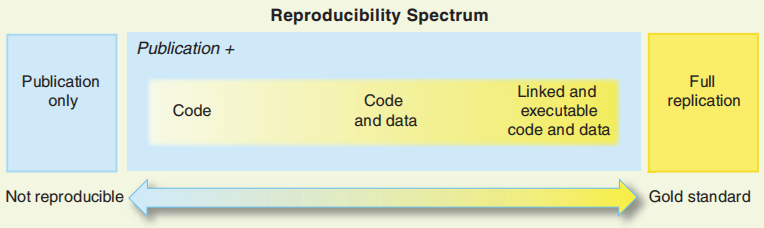
\includegraphics[width=.50\textwidth]{reproducibility_spectrum}
\caption[The spectrum of reproducibility.]{The spectrum of reproducibility (copyright by~\cite{peng2011reproducible}).}
\label{fig:reproducibility_spectrum}
\end{figure}



This chapter is divided in two parts. The first part (@todo) encloses the
systems and protocols we set in place in to make our research reproducible;
namely the \emph{iccvb} website and its public code repository. 
While the second part (@todo) describes the items to make our research
reproducible; namely the prostate dataset made available at \emph{iccvb},
the different toolboxes developed for and used in this thesis, as well the code
to replicate the experiments described in further chapters.

The aim of this chapter is two fold,
describe the systems and protocols we set
in place that make the research within this thesis reproducible. 


\section{Open Data - i2cvb website: an attempt to.. with a treat FREE (as sex, not beer) DATA}
\acs{iccvb} is a space we have created to deciminate our ideas about
reproducible research as stated by its four core pillars: 

\paragraph{Why?. our vision: to democratize the access to research}
The first need in modern research, regardless its application domain, is related to the access to reliable data for its subsequent study.

However, data gathering is an entrance barrier for most of the researchers mainly due to factors as diverse costs, infrastructure, availability, etc. Moreover, isolated endeavours to gather these data without granting public access lead to the creation of muda ("waste"): waste of resources and inability to compare results and validate conclusions.

Despite being highlighted by numerous research works, the lack of usable, public, reliable, and accessible data remains disregarded in many fields. The I2CVB is a wake-up call for addressing and breaking the entrance barriers in research due to data and/or isolation by applying collaborative strategies.

\paragraph{What?. mission: to democratize the access to research}
The lack of common data combined with non-aggregated assessing strategies result in non-existent or misleading comparisons make difficult to acknowledge relevant novel methodologies. A common duty to the research and development communities is to overcome these limitations, which can be successfully addressed by co-creation and collaborative work.

I2CVB aims at serving as foundation for collecting and sharing data as well as providing common evaluation methodologies. Furthermore, the use of common data and evaluation is the only way to achieve fair comparison.

\paragraph{Who?. protagonists: Research groups and individuals from all walks of life to shape a transparent community}
I2CVB creates for everyone the opportunity to pursue common goals through sharing, collaborating and team-working, to empower the individuals by taking advantages of personal skills and resources. As a consequence, young researchers will find an eco-system for self-improvement in which work will be rewarded through benchmarking compilation.

\paragraph{How?. strategy Transfer successful practises from Free Software and Quality Managemen}
I2CVB community challenges the impossible as well as the current status quo in research. Therefore, we strive to settle a multi-skilled community pursuing common goals to achieve excellence through collaborative continuous improvement.

At I2CVB, we believe that Free Software and Quality Management have already reshaped the world and that it is time to apply some of the successful practices learned in such domains to expand the boundaries of research in computer vision and specially for the medical imaging case.


\section{Open source}

All the different source code implemented for this thesis have been released to support future development and the possibility to build a consistent benchmark.
All available code is primarily developed in Python with a concern of:
(i) \emph{Quality insurance} by developing unit tests, automatic code quality checking, and code consistency checking using \texttt{PEP8} standards;
(ii) \emph{Continuous integration} is achieved through tools as Travis CI to easily integrate new contributions and ensure back-compatibility;
(iii) \emph{Community-based development} by using collaborative tools --- git, GitHub, and gitter --- to ease collaborative programming, issue tracking, code integration, and idea discussions;
(iv) \emph{Documentation} through a description of the developed API.

\section{Open \acs*{mpmri} data}

\paragraph{\SI{1.5}{\tesla} General Electric scanner}

The \ac{mpmri} data are acquired from a cohort of patients with higher-than-normal level of \ac{psa}.
The acquisition is performed using a \SI{1.5}{\tesla} whole body GE Signa \ac{mri} scanner (General Electric, Milwaukee, WI, USA) with an endorectal coil (Medrad, Pittsburgh, PA, USA), using sequences to obtain \ac{t2w}-\ac{mri}, \ac{dce}-\ac{mri}, \ac{dw}-\ac{mri}, and \ac{mrsi}.
Aside of the \ac{mri} examination, these patients also have undergone a guided-biopsy.
% The dataset is composed of a total of 20 patients of which 18 patients have biopsy proven \ac{cap} and 2 patients are ``healthy'' with negative biopsies.
% Therefore, 13 patients have a \ac{cap} in the \ac{pz}, 3 patients have \ac{cap} in the \ac{cg}, 2 patients have invasive \ac{cap} in both \ac{pz} and \ac{cg}, and finally 2 patients are considered as ``healthy''.
% An experienced radiologist has segmented the prostate organ as well as the prostate zones, and \ac{cap} on the \ac{t2w}-\ac{mri}.

Three-dimensional \ac{t2w} fast spin-echo (\ac{tr}/\ac{te}/\ac{etl}: \SI{3480}{\ms}/\SI{113.6}{\ms}/16, slice thickness: \SI{3}{\mm}) images are then acquired in an oblique axial plane with a  $320 \times 224$ acquisition matrix and a pixel spacing of \SI{0.27}{\milli\metre}.

%The nominal matrix and \ac{fov} of the 3D \ac{t2w} fast spin-echo images are \SI[product-units=repeat]{320x256}{\milli\metre\squared} and \SI[product-units=repeat]{280x240}{\milli\metre\squared}, respectively, thereby affording sub-millimetric pixel resolution within the imaging plane.

\ac{dce}-\ac{mri} is performed using a fat suppressed 3D fast spoiled gradient echo (\ac{tr}/\ac{te}/Flip angle: \SI{4.42}{\ms}/\SI{2.10}{\ms}/\SI{12}{\degree}; Matrix: $320 \times 192$; slab of 40 partitions of \SI{3.5}{\mm} thickness; temporal resolution: \SI{10}{\s}/slab over approximately \SI{5}{\minute}).
A power injector (Medrad, Indianola, USA) is used to provide a bolus injection of Gd-DTPA (Dotarem, Guerbet, Roissy, France) at a dose of \SI{0.2}{\ml} Gd-DTPA/kg of body weight.

\ac{dw}-\ac{mri} images have been acquired using the single-shot spin-echo echo-planar imaging (EPI) technique.
The diffusion-encoding gradients have been applied using a pulsed gradient spin-echo technique resulting in diffusion images acquired at 2 b-values --- i.e., \SI{100}{\second\per\milli\meter\squared} and \SI{1400}{\second\per\milli\meter\squared} --- and in the 3 orthogonal directions.
Sequential sampling of the k-space has been used with a \ac{te} of \SI{100.1}{\ms}, a \ac{tr} of \SI{10825}{\ms}, a bandwidth of \SI{1953}{\hertz\per\px}, and an acquisition matrix size of $128 \times 128$.

\ac{mrsi} is performed using a water and lipid suppressed double-spin-echo point-resolved spectroscopic (PRESS) sequence optimized for quantification detection of choline and citrate metabolites.
Water and lipid have been suppressed using a dual-band spectral spatial pulse technique.
%In order to eliminate signals from adjacent tissues, especially periprostatic lipids and the rectal wall up to 8 outer voxel saturation pulses have been used.
Datasets have been acquired as $16 \times 8 \times 8$ phase-encoded spectral arrays, a \ac{te} of \SI{130}{\ms}, a \ac{tr} of \SI{1000}{\ms}.%, and \SI{13}{\minute} of acquisition time.
%A spectral bandwidth of \SI{1250}{\hertz} has been used with 512 data points.
%A combination of an elliptic weighted averaged k-space acquisition scheme 3D filtering of the signal in k-space have been used, the latter in order to reduce intervoxel signal combination.
%Shimming has been carried out using the Siemenbens 3D Mapshim routine on a voxel adapted to the volume of the entire prostate gland.

\paragraph{\SI{3}{\tesla} Siemens scanner}

The \ac{mpmri} data are acquired from a cohort of patients with higher-than-normal level of \ac{psa}.
The acquisition is performed using a \SI{3}{\tesla} whole body \ac{mri} scanner (Siemens Magnetom Trio TIM, Erlangen, Germany) using sequences to obtain \ac{t2w}-\ac{mri}, \ac{dce}-\ac{mri}, \ac{dw}-\ac{mri}, and \ac{mrsi}.
Aside of the \ac{mri} examination, these patients also have undergone a guided-biopsy.
The dataset is composed of a total of 20 patients of which 18 patients have biopsy proven \ac{cap} and 2 patients are ``healthy'' with negative biopsies.
Therefore, 13 patients have a \ac{cap} in the \ac{pz}, 3 patients have \ac{cap} in the \ac{cg}, 2 patients have invasive \ac{cap} in both \ac{pz} and \ac{cg}, and finally 2 patients are considered as ``healthy''.
An experienced radiologist has segmented the prostate organ --- on \ac{t2w}-\ac{mri}, \ac{dce}-\ac{mri}, and \ac{adc}-\ac{mri} --- as well as the prostate zones --- i.e., \ac{pz} and \ac{cg} ---, and \ac{cap} on the \ac{t2w}-\ac{mri}.

A \SI{3}{\mm} slice fat-suppressed \ac{t2w} fast spin-echo sequence (\ac{tr}/\ac{te}/\ac{etl}: \SI{3400}{\ms}/\SI{85}{\ms}/13) is used to acquire images in sagittal and oblique coronal planes, the latter planes being orientated perpendicular or parallel to the prostate \ac{pz} – rectal wall axis.
Three-dimensional \ac{t2w} fast spin-echo (\ac{tr}/\ac{te}/\ac{etl}: \SI{3600}{\ms}/\SI{143}{\ms}/109, slice thickness: \SI{1.25}{\mm}) images are then acquired in an oblique axial plane.
The nominal matrix and \ac{fov} of the 3D \ac{t2w} fast spin-echo images are \SI[product-units=repeat]{320x256}{\milli\metre\squared} and \SI[product-units=repeat]{280x240}{\milli\metre\squared}, respectively, thereby affording sub-millimetric pixel resolution within the imaging plane.

\ac{dce}-\ac{mri} is performed using a fat suppressed 3D T$_1$ VIBE sequence (\ac{tr}/\ac{te}/Flip angle: \SI{3.25}{\ms}/\SI{1.12}{\ms}/\SI{10}{\degree}; Matrix: $256 \times 192$; \ac{fov}: $280 \times 210$ (with \SI{75}{\percent} rectangular \ac{fov}); slab of 16 partitions of \SI{3.5}{\mm} thickness; temporal resolution: \SI{6}{\s}/slab over approximately \SI{5}{\minute}).
A power injector (Medrad, Indianola, USA) is used to provide a bolus injection of Gd-DTPA (Dotarem, Guerbet, Roissy, France) at a dose of \SI{0.2}{\ml} Gd-DTPA/kg of body weight.

\ac{dw}-\ac{mri} images have been acquired using the single-shot spin-echo echo-planar imaging (EPI) technique.
As proposed by \citeauthor{stejskal1965spin}~\cite{stejskal1965spin}, the diffusion-encoding gradients have been applied using a pulsed gradient spin-echo technique resulting in diffusion images acquired at 2 b-values --- i.e., \SI{100}{\second\per\milli\meter\squared} and \SI{800}{\second\per\milli\meter\squared} --- and in the 3 orthogonal directions.
Sequential sampling of the k-space has been used with a \ac{te} of \SI{101}{\ms}, a \ac{tr} of \SI{4200}{\ms}, and a bandwidth of \SI{1180}{\hertz\per\px}.
Other parameters included a \ac{fov} of \SI{240}{\milli\metre}, an acquisition matrix size of $128 \times 128$ and a slice thickness of \SI{3.5}{\milli\metre}.
The \ac{adc} map has been directly generated by the Siemens workstation from the raw data on a pixel-by-pixel basis.

\ac{mrsi} is performed using a water and lipid suppressed double-spin-echo point-resolved spectroscopic (PRESS) sequence optimized for quantification detection of choline and citrate metabolites.
Water and lipid have been suppressed using a dual-band spectral spatial pulse technique.
In order to eliminate signals from adjacent tissues, especially periprostatic lipids and the rectal wall up to 8 outer voxel saturation pulses have been used.
Datasets have been acquired as $16 \times 12 \times 16$ --- interpolated to $16 \times 16 \times 16$ phase-encoded spectral arrays, a \ac{te} of \SI{140}{\ms}, a \ac{tr} of \SI{720}{\ms} and \SI{13}{\minute} of acquisition time.
A spectral bandwidth of \SI{1250}{\hertz} has been used with 512 data points.
A combination of an elliptic weighted averaged k-space acquisition scheme 3D filtering of the signal in k-space have been used, the latter in order to reduce intervoxel signal combination.
Shimming has been carried out using the Siemenbens 3D Mapshim routine on a voxel adapted to the volume of the entire prostate gland.
Additional unsuppressed water acquisitions at \ac{te} of \SI{30}{\ms}, \SI{80}{\ms}, and \SI{140}{\ms} of \SI{1.5}{\minute} have also been performed in order to allow quantification with respect to prostate water.
Systematic verification of the global shim --- i.e., over the complete 3D PRESS-selected volume --- revealed line widths at half-height of the water peak of the order of \SIrange{20}{30}{\hertz}, routinely.
The line widths for individual voxels are of the order of \SIrange{8}{12}{\hertz}.
The total examination time, including the time spent positioning the patient, is approximately 45 minutes.


\section{\texttt{imbalanced-learn} toolbox}

The \texttt{imbalanced-learn} toolbox is an open-source python toolbox aiming at providing a wide range of methods to cope with the problem of imbalanced dataset frequently encountered in machine learning and pattern recognition.
The implemented state-of-the-art methods can be categorized into 4 groups: (i) under-sampling, (ii) over-sampling, (iii) combination of over- and under-sampling, and (iv) ensemble learning methods.
The proposed toolbox only depends on \texttt{numpy}, \texttt{scipy}, and \texttt{scikit-learn} and is distributed under MIT license.
Furthermore, it is fully compatible with \texttt{scikit-learn} and is part of the \texttt{scikit-learn-contrib} supported project.
Documentation, unit tests as well as integration tests are provided to ease usage and contribution.
The toolbox is publicly available in GitHub\footnote{\url{https://github.com/scikit-learn-contrib/imbalanced-learn}}.

To illustrate the developed API and the compatibility with \texttt{scikit-learn}, an example of a pipeline using a \ac{pca} decomposition, a \ac{smote} over-sampler, and a \ac{knn} classifier is presented below:

\begin{lstlisting}[language=Python, caption=Code snippet to over-sample a dataset using \acs*{smote} in conjunction with \ac{pca} and a \ac{knn} classifer.]
from sklearn.datasets import make_classification
from sklearn.cross_validation import train_test_split as tts
from sklearn.decomposition import PCA
from sklearn.neighbors import KNeighborsClassifier as KNN
from sklearn.metrics import classification_report
from imblearn.over_sampling import SMOTE
from imblearn.pipeline import Pipeline
X, y = make_classification(n_classes=2, class_sep=2,
                           n_informative=3, n_redundant=1, flip_y=0,
                           n_features=20, n_clusters_per_class=1,
                           n_samples=1000, weights=[0.1, 0.9])
pca = PCA()
smt = SMOTE()
knn = KNN()
pipeline = Pipeline([('smt', smt), ('pca', pca), ('knn', knn)])
X_train, X_test, y_train, y_test = tts(X, y, random_state=42)
pipeline.fit(X_train, y_train)
y_hat = pipeline.predict(X_test)
\end{lstlisting}

\section{\texttt{protoclass} toolbox}

The \texttt{protoclass} toolbox is an open-source python toolbox providing tools for fast prototyping of machine learning pipeline in medical imaging.
It implements most of the state-of-the-art feature detection techniques presented in \acs{chp}\,\ref{chap:3}.
To illustrate the API, an example is given in which a \ac{t2w}-\ac{mri} volume is normalized and the voxels corresponding to the prostate are extracted and can be used easily with \texttt{scikit-learn}.

\begin{lstlisting}[language=Python, caption=Code snippet to normalize a volume and extract some voxels.]
import os
from protoclass.data_management import T2WModality
from protoclass.data_management import GTModality
from protoclass.preprocessing import GaussianNormalization
from protoclass.extraction import IntensitySignalExtraction

# Define the path the different data path
path_t2w = '/data/T2W'
path_gt = ['/data/GT/prostate']
label_gt = ['prostate']

# Read the T2W
t2w_mod = T2WModality()
t2w_mod.read_data_from_path(path_t2w)

# Read the ground-truth
gt_mod = GTModality()
gt_mod.read_data_from_path(label_gt, path_gt)

# Normalize the T2W modality
t2w_norm = GaussianNormalization(T2WModality())
t2w_norm.fit(t2w_mod, ground_truth=gt_mod, cat=label_gt[0])
t2w_mod = t2w_norm.normalize(t2w_mod, ground_truth=gt_mod,
                             cat=label_gt[0])

# Extract the voxel from the prostate
ise = IntensitySignalExtraction(t2w_mod)
data = ise.transform(t2w_mod, ground_truth=gt_mod, cat=label_gt[0])
\end{lstlisting}

\section{Pipeline-data releases}

	
\chapter{Normalization/Standardization of T2W-MRI and DCE-MRI Images} \label{chap:5}
\Ac{cad} systems are usually designed as a sequential process consisting of four stages: pre-processing, segmentation, registration, and classification.
We presented in \acs{sec}\,\ref{subsubsec:ch3:mriprepro} the state-of-the-art techniques for normalization/standardization of \ac{mri} modality among other pre-processing steps.
As a conclusion, we can stress that only little attention has been dedicated to this topic.
Data normalization is, however, a crucial and important step of the chain to design a robust classifier and overcome the inter-patient intensity variations.

In this chapter, we focus on the normalization of \ac{t2w}-\ac{mri} and \ac{dce}-\ac{mri} modalities.
On the one hand, we investigate two \ac{t2w}-\ac{mri} normalization methods based on (i) Rician \emph{a priori} and (ii) \ac{srsf} representation and compare them with the state-of-the-art methods.
On the other hand, we propose and investigate a fully automated framework for \ac{dce}-\ac{mri} normalization, the first of its kind.

\section{Normalization of \ac{t2w}-\ac{mri} images} \label{sec:chp5:T2-norm}

This section focuses on \ac{t2w}-\ac{mri} normalization.
First, the related work is presented in \ac{sec}\,\ref{subsec:chp5:relwork1} before to focus on two new normalization methods which are presented and investigated in \acs{sec}\,\ref{subsec:chp5:T2-norm:meth} and \acs{sec}\,\ref{subsec:chp5:T2-norm:Exp-res}

\subsection{Related work}\label{subsec:chp5:relwork1}

We briefly recall the state-of-the-art methods which have been proposed for the normalization of \ac{t2w}-\ac{mri} prostate images.

\citeauthor{Artan2010}, \citeauthor{Ozer2010}, and \citeauthor{rampun2016computerb} used a parametric method to normalize \ac{t2w}\ac{mri} images~\cite{Artan2009,Artan2010,Ozer2009,Ozer2010,rampun2015classifying,rampun2015computer,rampun2016computer,rampun2016computerb}.
This parametric method is based on computing the standard score --- also known as \emph{z-score} --- of the \ac{pz} voxels such as: 
\begin{equation}
  I_{s}(x) = \frac{I_{r}(x) - \mu_{PZ}}{\sigma_{PZ}}, \forall x\in PZ ,
  \label{eq:zscore}
\end{equation}
\noindent where, $I_{s}(x)$ and $I_{r}(x)$ are the standardized and the raw signal intensity, respectively, and $\mu_{PZ}$ and $\sigma_{PZ}$ are the mean and standard deviation of the \ac{pz} signal intensity, respectively. 
This transformation enforces the image \ac{pdf} to have a null mean and a unit standard deviation.
However, this normalization is not appropriate if the \ac{pdf} do not follow a Gaussian distribution as illustrated in Fig.\,\ref{fig:fitting}

\citeauthor{Lv2009}~cite{Lv2009} used the non-parametric method which is a piecewise-linear normalization, proposed by \citeauthor{Nyul2000} in~\cite{Nyul2000}.
For a given patient, a warping function is inferred by matching some specific landmarks --- i.e., different percentiles --- of the current \ac{pdf} to the same landmarks learned during a training phase from several patients. 
The mapping between each landmark is performed using a linear mapping.
\citeauthor{Viswanath2012} used a variant of the previous method by segmenting first the image using region growing with a pre-defined homogeneity criterion and keeping only the largest region to build the \ac{pdf}~\cite{Viswanath2012}.
Nevertheless, the warping functions inferred by these methods suffer from abrupt changes --- refer to \acs{fig}\,\ref{fig:maplinear} --- around the landmarks position, leading to a disrupt \ac{pdf} in the normalized image.

In this section, we evaluate and compare different normalization approaches in the context of \ac{t2w}-\ac{mri} prostate image normalization.
Our contribution is threefold: (i) a parametric normalization approach based on a Rician \textit{a priori}; (ii) a non-parametric normalization approach based on a method used in registration of functional data; and (iii) a novel evaluation metric to asses quantitatively the alignment of the \acp{pdf} independently of the assumed distribution. 
These methods are compared qualitatively and quantitatively, with both \textit{z-score} normalization and piecewise-linear normalization.

\subsection{Methodology}\label{subsec:chp5:T2-norm:meth}

\subsubsection{Parametric normalization using Rician \textit{a priori}}\label{subsubsec:chp5:T2-norm:meth:rician}
As previously stated, proper normalization of the \ac{mri} data during pre-processing is a key problem that has been addressed using parametric and non-parametric strategies.
We believe that normalizing \ac{mri} data using a parametric model based on a Rician distribution would improve the results.
Expecting this improvement by changing the data model from the widely used Gaussian distribution to Rician distribution is reasonable.
Indeed, \citeauthor{Bernstein1989} state that \ac{mri} data theoretically follow a Rayleigh distribution for a low-\ac{snr} scenarios while it appears closer to a Gaussian distribution when the \ac{snr} increases~\citeauthor{Bernstein1989}.
Figure~\ref{fig:fitting} shows the intensity spectrum for some \ac{mri} prostate data as well as the fitted Gaussian and Rician distributions.
A qualitative assessment of the underlying distribution is performed by overlying the fitted distribution, while quantitative results of the fitting are given in terms of \ac{rms}.
It can be highlighted that the Rician model better fits the data than the Gaussian model.

\begin{figure}
  \centering
  \subfigure[]{
    \label{fig:p1}\includegraphics[width=0.48\textwidth]{5_normalization/figures/T2-normalization/03}}\hfill
  \subfigure[]{
    \label{fig:p2}\includegraphics[width=0.48\textwidth]{5_normalization/figures/T2-normalization/06}}\hfill
%  \subfloat[][]{
%    \label{fig:p3}\includegraphics[width=0.3\textwidth]{14}}
  \caption{Visual evaluation of the goodness of fitting using Rician and Gaussian distribution.}
  \label{fig:fitting}
\end{figure}

The normalization is carried out through the following 3 steps: 
(i) fit a Rician model --- \acs{eq}\,\eqref{eq:rice} --- to each prostate \ac{pdf} using non-linear least squares minimization, namely Levenberg-Marquardt; 
(ii) compute the mean --- \acs{eq}\,\eqref{eq:meanr} --- and variance --- \acs{eq}\,\eqref{eq:var} --- of the Rician model;
(iii) normalize the entire data using the \textit{z-score} similarly as in~\acs{eq}\,\eqref{eq:zscore}.

\begin{equation}
  f(x| \nu, \sigma) = \frac{x}{\sigma^2}\exp\left( \frac{- (x^2 + \nu^2)}{2\sigma^2} \right) I_0 \left( \frac{x \nu}{\sigma^2} \right) \ ,
  \label{eq:rice}
\end{equation}

\begin{equation}
  \mu_{r} = \sigma  \sqrt{\frac{\pi}{2}}\,\,L_{1/2}(-\frac{\nu^2}{2\sigma^2})  \ ,
  \label{eq:meanr}
\end{equation}

\begin{equation}
  \sigma_{r} = 2\sigma^2+\nu^2-\frac{\pi\sigma^2}{2}L_{1/2}^2\left(\frac{-\nu^2}{2\sigma^2}\right)  \ ,
  \label{eq:var}
\end{equation}

\noindent where $\nu$ and $\sigma$ are the distance between the reference point and the center of the bi-variate distribution and the scale, respectively; $L_{1/2}$ denotes a Laguerre polynomial; $I_0$ is the modified Bessel function of the first kind with order zero.

\subsubsection{Non-parametric normalization based on \acs*{srsf}}\label{subsubsec:chp5:T2-norm:gen-model}

\citeauthor{Srivastava2011} proposed a generic method to register functional data, without any assumption regarding the models of the different functions~\cite{Srivastava2011}. 
In a nutshell, this framework relies on the \ac{srsf} representation which transforms the Fisher-Rao metric into the conventional $\mathbb{L}^2$ metric, and thus allows to define a cost function corresponding to an Euclidean distance between 2 functions in this new representation.

\paragraph{\Ac{srsf} representation}

In the proposed registration framework of functional data, 2 functions $f_1$ and $f_2$ are registered by composing $f_2$ with a warping function $\gamma$ such that:

\begin{equation}
  \argmin_{\gamma \in \Gamma} D_{FR}(f_1, (f_2 \circ \gamma)) \ ,
  \label{eq:regfun}
\end{equation}

\noindent where $D_{FR}$ is the Fisher-Rao distance and $\Gamma$ is the set of all the functions $\gamma$.

The \ac{srsf} representation is used to transform the functions and register them into this space.
The \ac{srsf} of a function $f$ is defined as:

\begin{equation}
  q(t) = \sign(\dot{f}(t))\sqrt{|\dot{f}(t)|} \ ,
  \label{eq:srsf}
\end{equation}

\noindent where $\dot{f}(t)$ corresponds to the derivative of $f$.

The major property of the \ac{srsf} representation used in the registration framework is the following: the composition of a function $f$ with a warping function $\gamma$ --- i.e., $f \circ \gamma$ --- is equivalent to \acs{eq}\,\eqref{eq:warp}, using the \ac{srsf} representation.

\begin{equation}
  \tilde{q}(t) = (q(t) \circ \gamma) \sqrt{\dot{\gamma}} \ ,
  \label{eq:warp}
\end{equation}

\noindent where $\dot{\gamma}$ is the derivative of $\gamma$.

Using this property, a cost function --- so called amplitude or $y$-distance --- is defined to measure the similarity between the 2 functions $f_1$ and $f_2$, expressed as in \acs{eq}\,\eqref{eq:cf}

\begin{equation}
  D_y(f_1, f_2) = \underset{\gamma \in \Gamma}{\infspie} \| q_1 - (q_2 \circ \gamma) \sqrt{\dot{\gamma}} \| \ .
  \label{eq:cf}
\end{equation}

\paragraph{Registration framework}\label{par:chp5:T2-norm:regfra}

The registration framework consists of 2 steps.
First, an initialization in which the Karcher mean $\mu_f$ is computed as in \acs{eq}\,\eqref{eq:mean}

\begin{equation}
  \mu_f = \argmin_{f \in \mathcal{F}} \sum_{i = 1}^{n} D_y(f, f_i)^2 \ .
  \label{eq:mean}
\end{equation}

Then, for each function $f_i$: 
(i) compute $\gamma_{i}^{*}$ as in \ac{eq}\,\eqref{eq:warpi}; 
(ii) compute $\tilde{q}_i$ as in \ac{eq}\,\eqref{eq:warp};
(iii) update $\mu_f$ as in \ac{eq}\,\eqref{eq:mean} by replacing $f_i$ by $\tilde{f_i}$, using $\tilde{q}_i$.

\begin{equation}
  \gamma_{i}^{*} = \argmin_{\gamma \in \Gamma} \sum_{i = 1}^{n} D_y(\mu_f, f_i)^2 \ ,
  \label{eq:warpi}
\end{equation}

\noindent where $n$ is the total number of functions to be aligned.

This step is performed in an iterative manner based on the gradient of the cost function given in \acs{eq}\,\eqref{eq:mean}. 
We refer the reader to the work of \citeauthor{Srivastava2011} for more detailed discussion~\cite{Srivastava2011}.

\subsubsection{Evaluation metric}

In their work, \citeauthor{Nyul2000} evaluated the normalization methods by computing the variation of the mean of a specific tissue.
However, this measure can be biased since that the mean can also be used as a landmark with the piecewise-linear method.
Furthermore, considering a single statistic does not allow to evaluate the overall performance of a normalization.
Indeed, this statistic corresponds to evaluate a single point of the mapping function and thus a large portion of the mapping functions are disregarded. 

That is why, to evaluate the performance of the different metric, we propose to use a spectral evaluation by decomposing the set of normalized \ac{pdf}s using \ac{pca} under the assumption that they are linearly dependent. 
Intuitively, the eigenvalues of the \ac{pca} decomposition are correlated with the alignment of the different \acp{pdf}.
Thus, in the case of a perfect alignment of the \ac{pdf}s, the first eigenvalue is much greater than the remaining since that the first eigenvector encodes all the information.
In the contrary, in the case of a misalignment of the \ac{pdf}s, more eigenvectors are needed to encode the information synonymous with larger eigenvalues.
Therefore, the cumulative sum of the normalized eigenvalues as well as the \ac{auc} are used, as depicted in \acs{fig}\,\ref{fig:qt}.

\subsection{Materials}\label{subsec:chp5:T2-norm:Exp-res}

The experiments are conducted on a subset of the public \ac{mpmri} prostate presented in \acs{sec}\,\ref{chp4:sec:data}.
We used the \SI{3}{\tesla} dataset which is composed of a total of 20 patients of which 18 patients had biopsy proven \ac{cap} and 2 patients are ``healthy'' with negative biopsies. 
In this study, our subset consists of 17 patients with \ac{cap}.

The different normalization methods are implemented in Python and are part of the \texttt{protoclass} toolbox presented in \acs{sec}\,\ref{chp4:sec:data}.
The normalization based on \ac{srsf} uses the implementation\footnote{\url{https://bitbucket.org/tetonedge/fdasrsf}} of \citeauthor{Tucker2013}~\cite{Tucker2013}.
The piecewise-linear normalization is performed using the following set of percentiles $s \in \{0, 5, 25, 50, 75, 95, 100 \}$ as landmarks.
In the \ac{srsf}-based normalization, the \acp{pdf} are smoothed using spline-based denoising method.

\subsection{Results and discussion}

\paragraph{Qualitative results}

% \begin{figure}
%   \centering
%   \includegraphics[width=1.\textwidth]{5_normalization/figures/T2-normalization/qualitative.png}
%   \caption{Qualitative evaluation by visual inspection of the alignment of the \ac{pdf}s for the full prostate and the \ac{cap}.}
%   \label{fig:qu}
% \end{figure}

\begin{figure}
  \hspace*{\fill}
  \subfigure[Piecewise-linear mapping function.]{
    \label{fig:maplinear}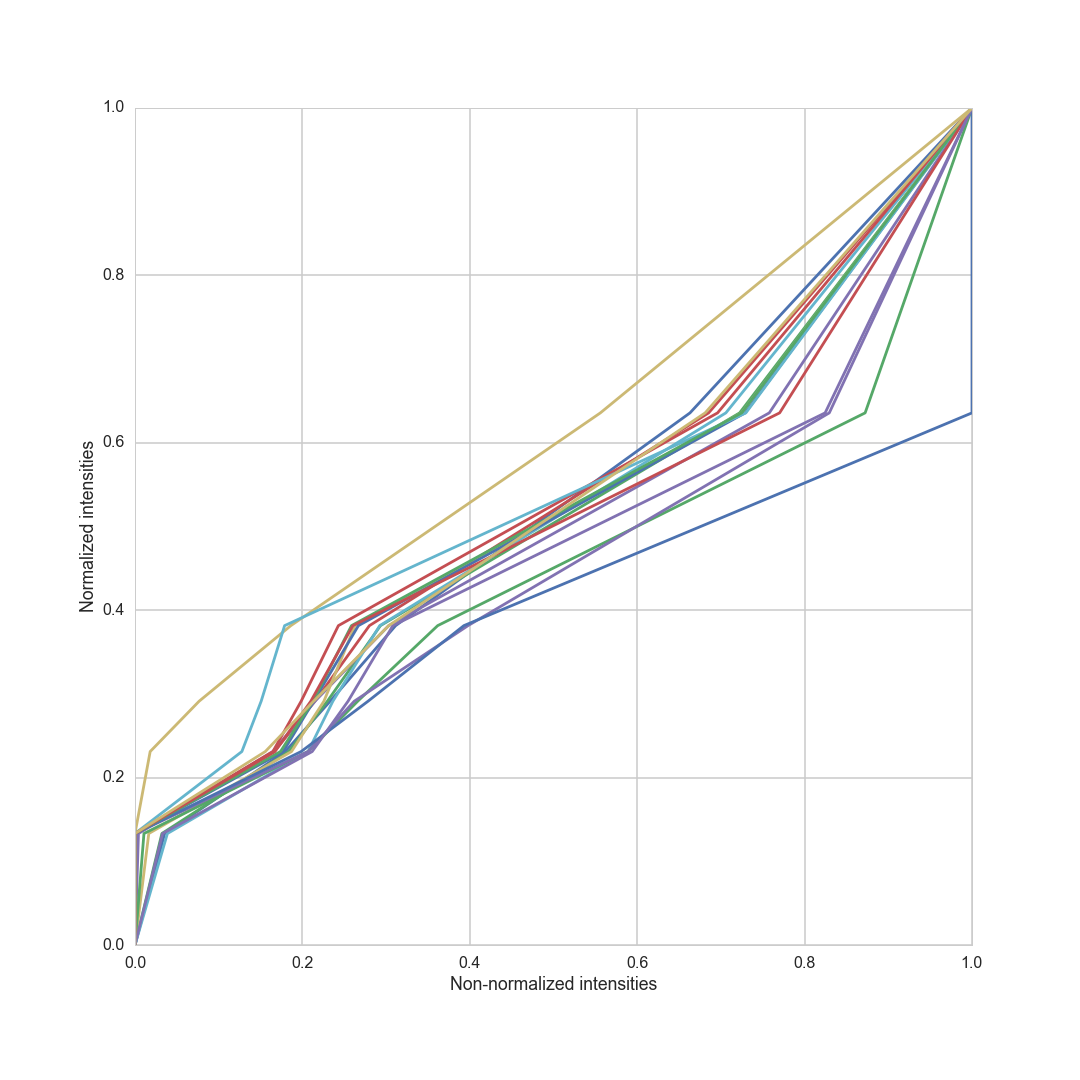
\includegraphics[width=0.4\textwidth]{5_normalization/figures/T2-normalization/piecewise-linear.png}}\hfill
  \subfigure[\acs*{srsf} mapping function.]{
    \label{fig:mapsrsf}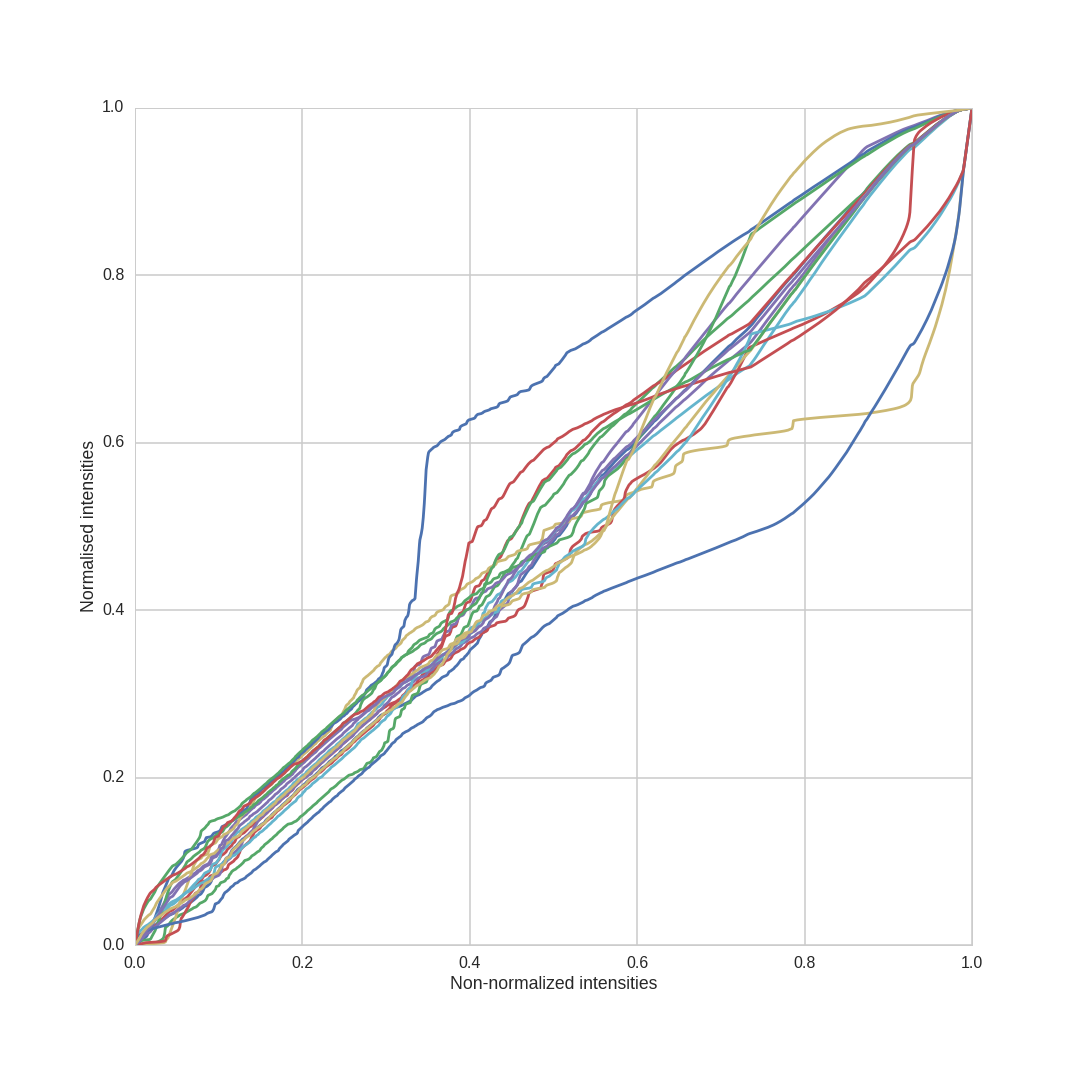
\includegraphics[width=0.4\textwidth]{5_normalization/figures/T2-normalization/srsf.png}}
  \hspace*{\fill}
  \caption[Comparison of the mapping functions found with the piecewise-linear and \acs{srsf}-based normalization.]{Comparison of the mapping functions found with the piecewise-linear and \acs{srsf}-based normalization. Each curve corresponds to a mapping function for a single patient.}
  \label{fig:mapping}
\end{figure}

\Acl{fig}~\ref{fig:qu} depicts the alignment of the different \acp{pdf} using the different methods implemented. 
All the methods seem to address the problem of the \ac{pdf} alignment of the full prostate data.
However, the Rician normalization outperforms the other methods when focusing solely on the \ac{cap} data.
The \ac{pdf} computed in this specific area is more skewed from its original shape in the case of the piecewise-linear normalization than with the 3 other normalization strategies.
The \ac{srsf} normalization gets unstable due to the warping function $\gamma$ found which is in practise non-smooth as shown in \acs{fig}\,\ref{fig:mapsrsf}.

\begin{landscape}

\begin{figure}
  \hspace*{\fill}
  \subfigure[Raw prostate.]{
    \label{subfig:raw}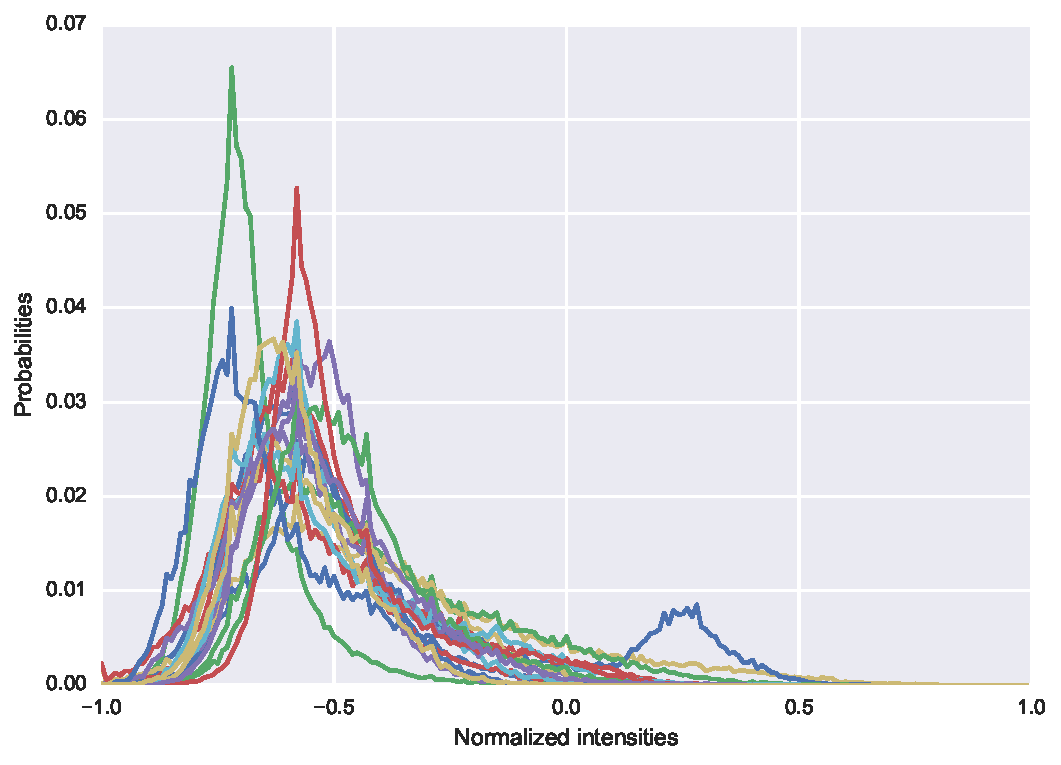
\includegraphics[width=.23\linewidth]{5_normalization/figures/T2-normalization/raw.pdf}}
  \hfill
  \subfigure[Raw \acs*{cap}]{
    \label{subfig:raw_cap}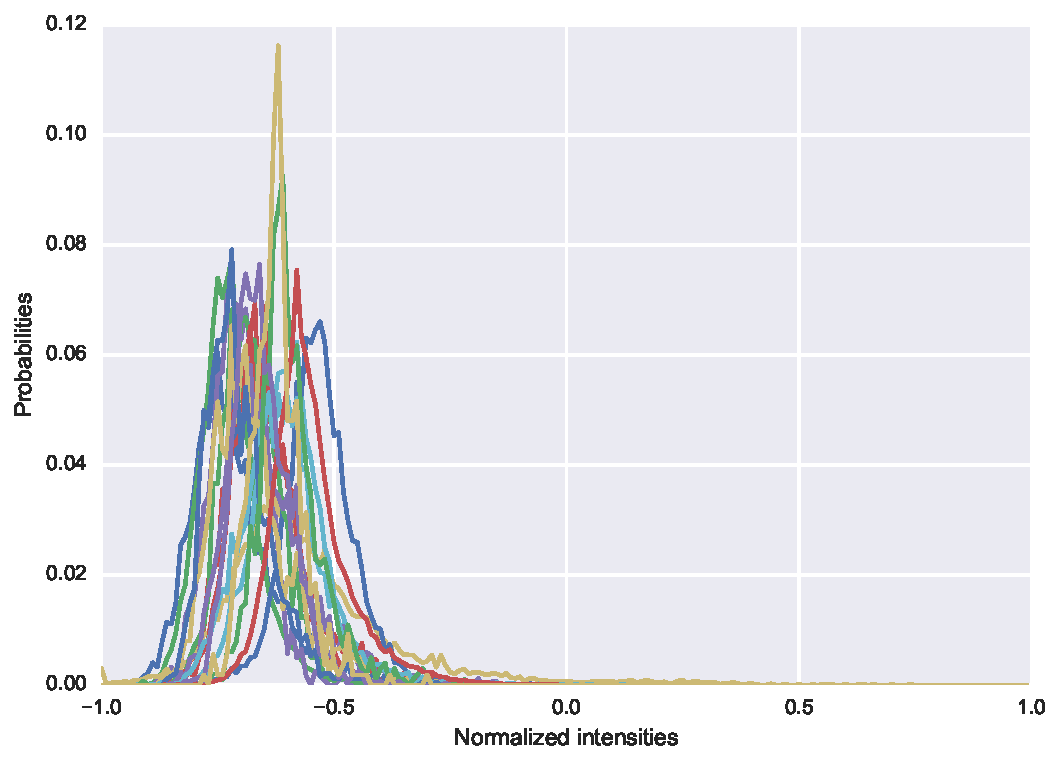
\includegraphics[width=.23\linewidth]{5_normalization/figures/T2-normalization/raw_cap.pdf}}
  \hspace*{\fill}
  \\
  \hspace*{\fill}
  \subfigure[Gaussian prostate.]{
    \label{subfig:gaussian}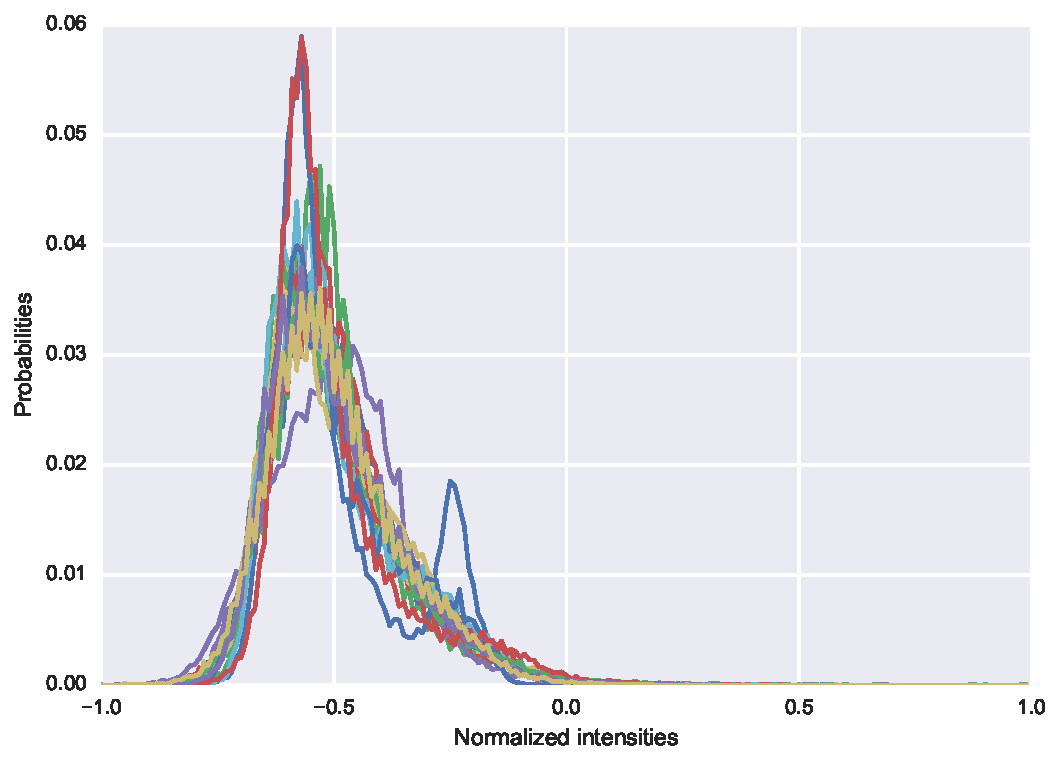
\includegraphics[width=.23\linewidth]{5_normalization/figures/T2-normalization/gaussian.pdf}}
  \hfill
  \subfigure[Rician prostate.]{
    \label{subfig:rician}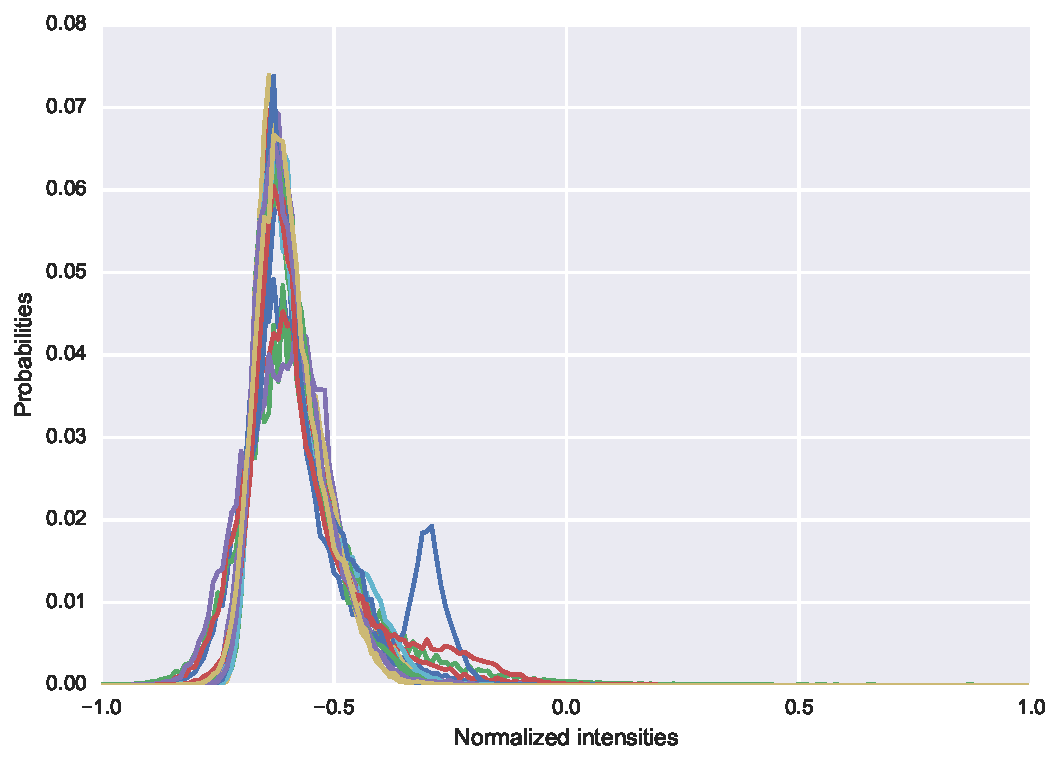
\includegraphics[width=.23\linewidth]{5_normalization/figures/T2-normalization/rician.pdf}}
  \hfill
  \subfigure[Linear prostate.]{
    \label{subfig:piecewise}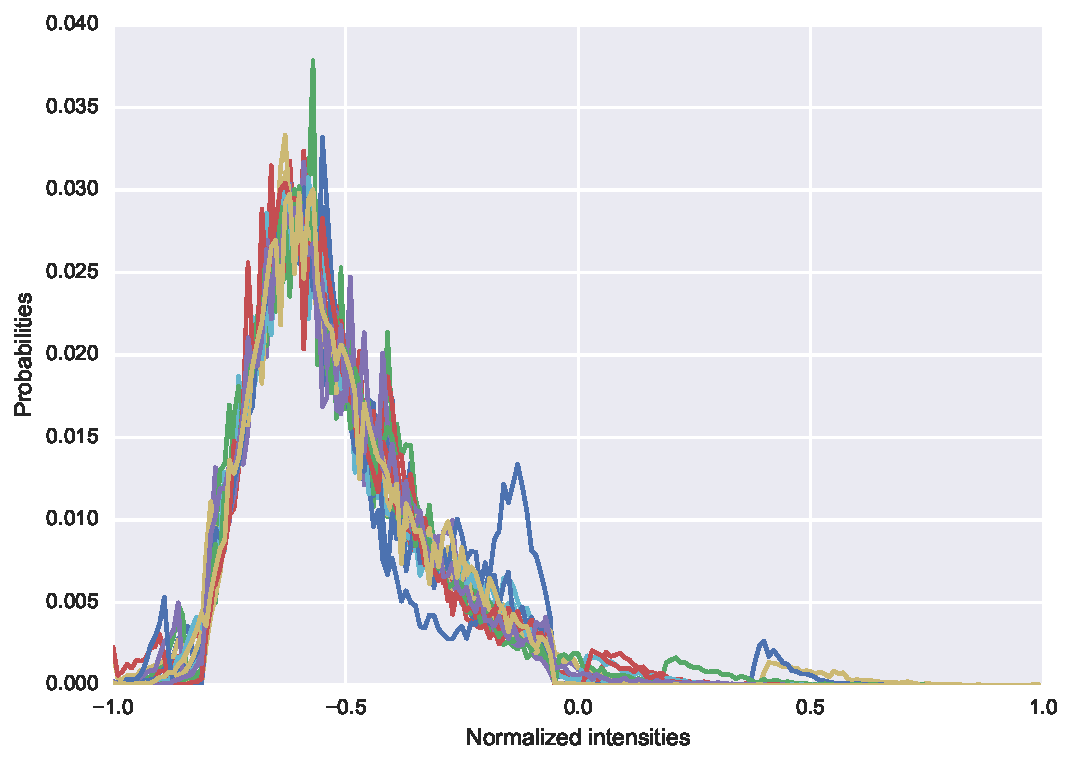
\includegraphics[width=.23\linewidth]{5_normalization/figures/T2-normalization/piecewise.pdf}}
  \hfill
  \subfigure[\acs*{srsf} prostate.]{
    \label{subfig:srsf}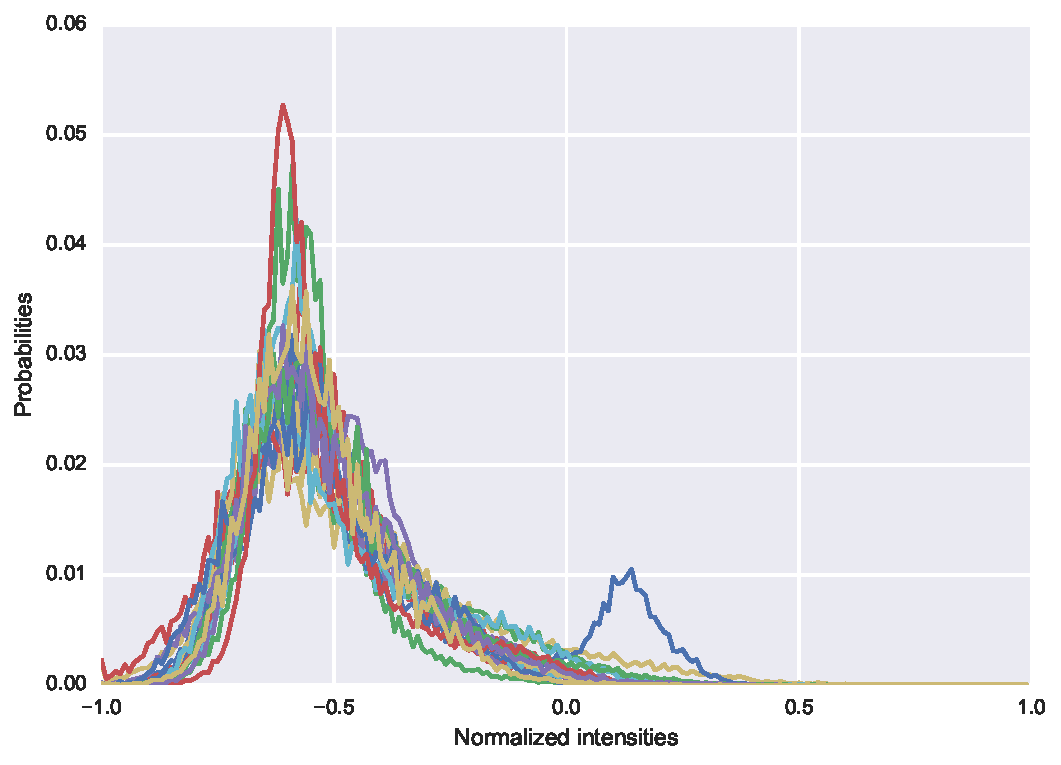
\includegraphics[width=.23\linewidth]{5_normalization/figures/T2-normalization/srsf.pdf}}
  \hspace*{\fill}\\
  \hspace*{\fill}
  \subfigure[Gaussian \acs*{cap}.]{
    \label{subfig:gaussian_cap}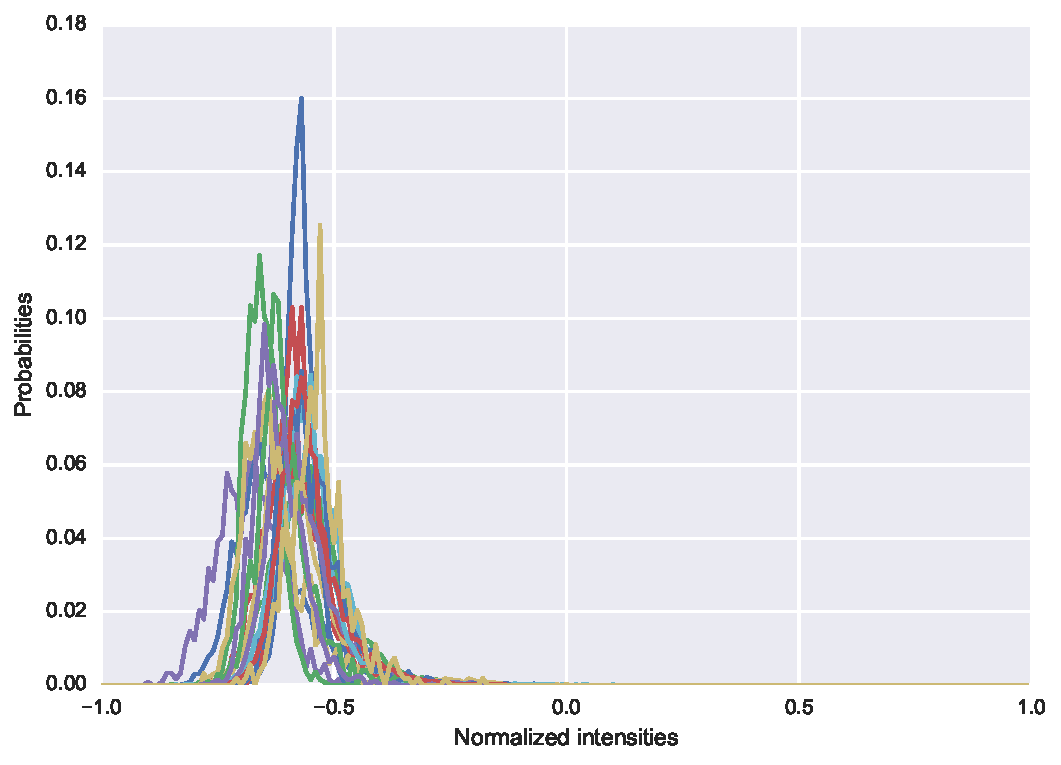
\includegraphics[width=.23\linewidth]{5_normalization/figures/T2-normalization/gaussian_cap.pdf}}
  \hfill
  \subfigure[Rician \acs*{cap}.]{
    \label{subfig:rician_cap}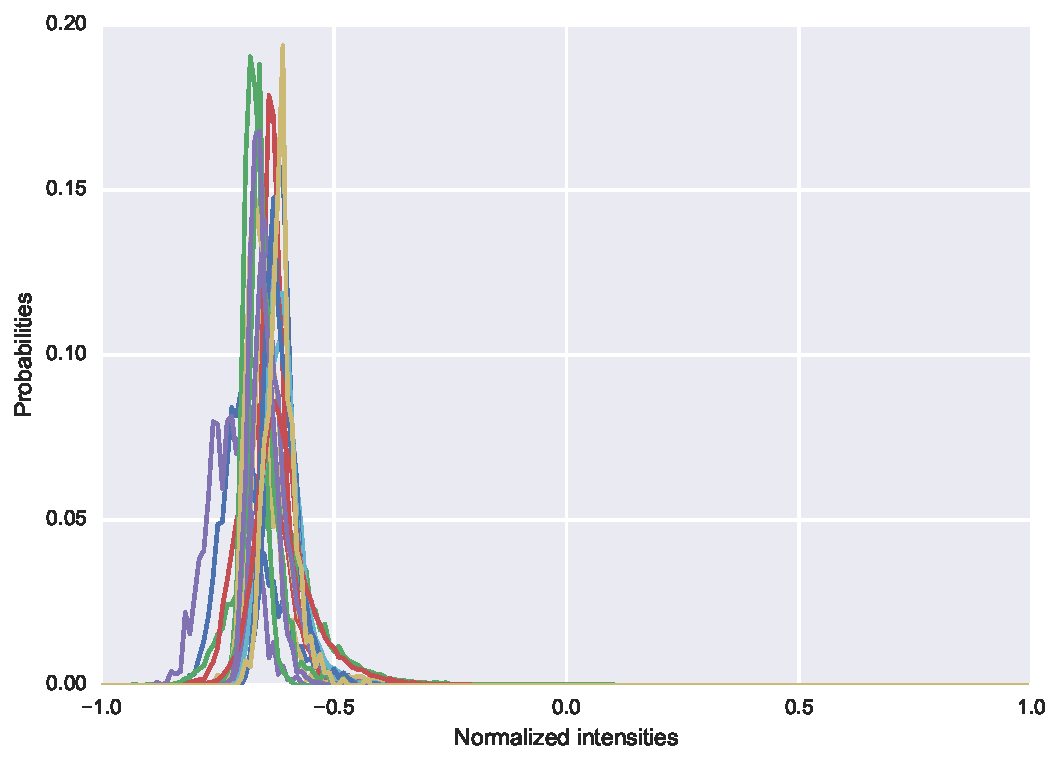
\includegraphics[width=.23\linewidth]{5_normalization/figures/T2-normalization/rician_cap.pdf}}
  \hfill
  \subfigure[Linear \acs*{cap}.]{
    \label{subfig:piecewise_cap}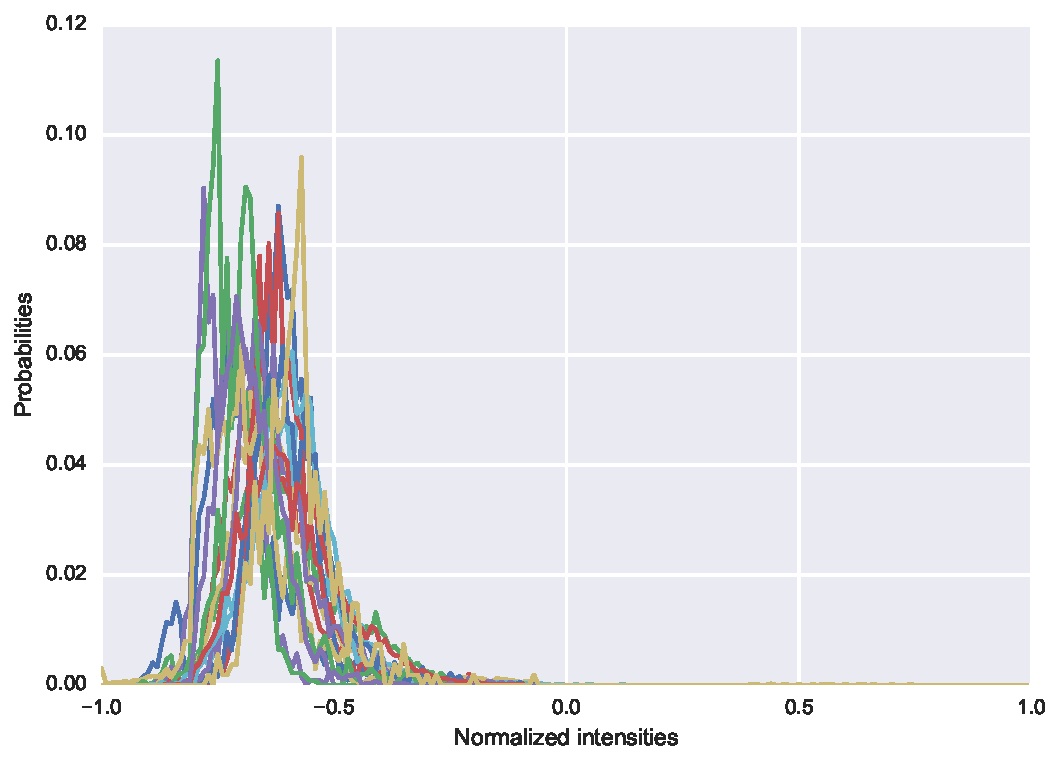
\includegraphics[width=.23\linewidth]{5_normalization/figures/T2-normalization/piecewise_cap.pdf}}
  \hfill
  \subfigure[\acs*{srsf} \acs*{cap}.]{
    \label{subfig:srsf_cap}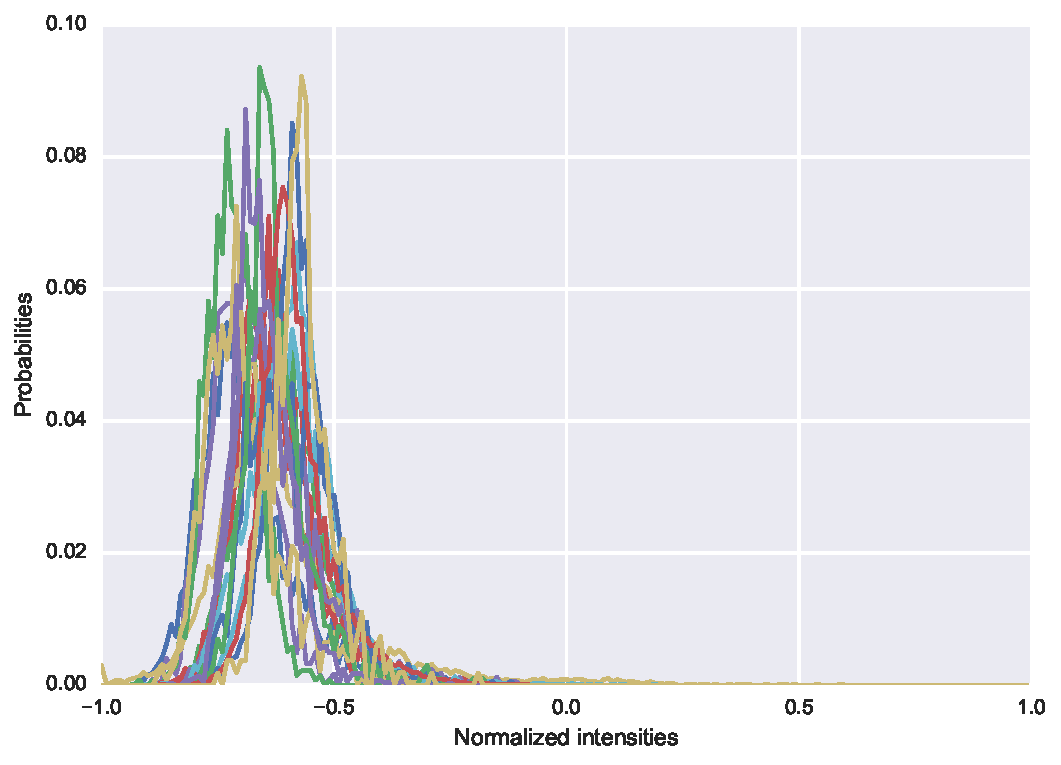
\includegraphics[width=.23\linewidth]{5_normalization/figures/T2-normalization/srsf_cap.pdf}}
  \hspace*{\fill}
  \caption[Qualitative valuation for \acs*{t2w}-\acs*{mri}]{Qualitative evaluation by visual inspection of the alignment of the \acs*{pdf}s for the full prostate and the \acs*{cap} in \acs*{t2w}-\acs*{mri}. The first row corresponds to the original \acs*{pdf}}
  \label{fig:qu}
\end{figure}

\end{landscape}

\paragraph{Quantitative results}

\begin{figure}
  \centering
  \subfigure[]{
    \label{fig:qtfull}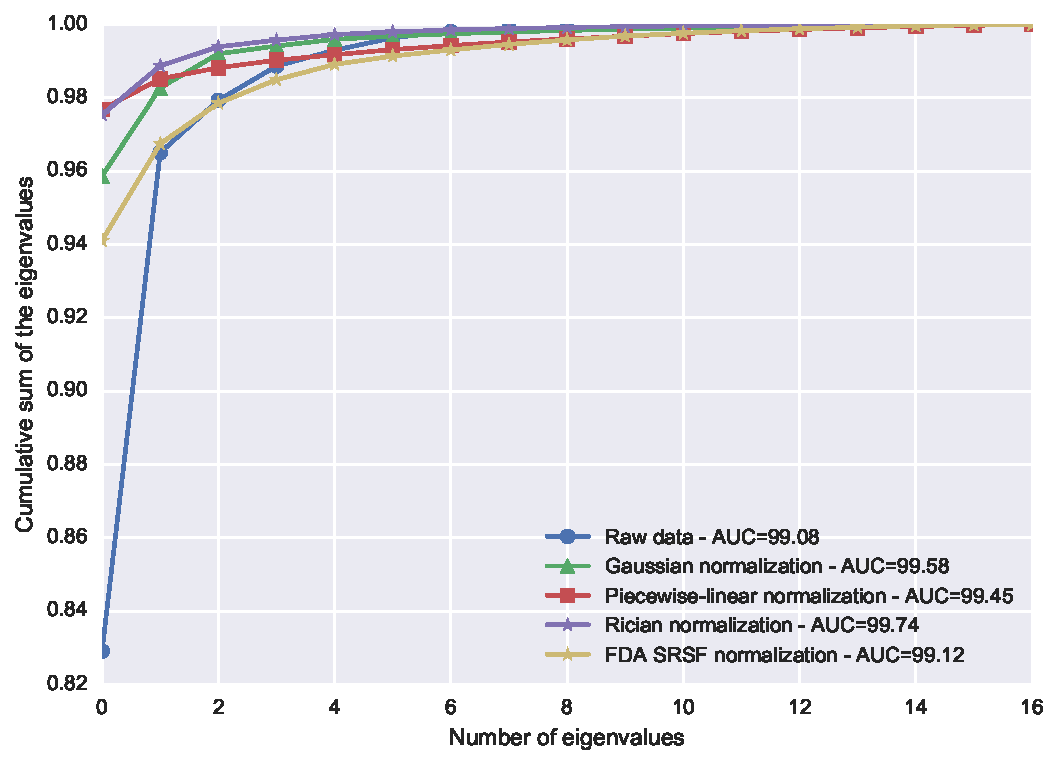
\includegraphics[width=0.8\textwidth]{5_normalization/figures/T2-normalization/quantitative_1.pdf}}\\
  \subfigure[]{
    \label{fig:qtcap}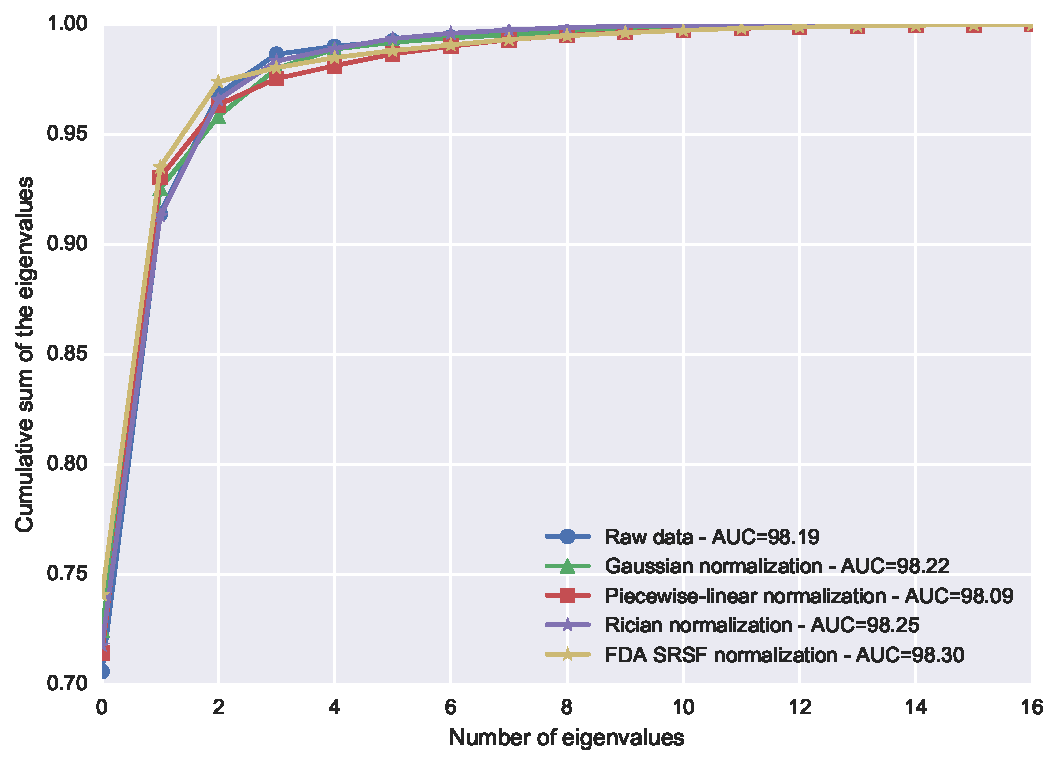
\includegraphics[width=0.8\textwidth]{5_normalization/figures/T2-normalization/quantitative_2.pdf}}
  \caption{Spectral evaluation using \ac{pca} decomposition: \protect\subref{fig:qtfull} evaluation considering the full prostate, \protect\subref{fig:qtcap} evaluation considering only the \ac{cap}.}
  \label{fig:qt}
\end{figure}

In overall, all normalization methods improve the alignment of the \acp{pdf}.
The parametric methods outperform the non-parametric while evaluating the \ac{pdf} alignment considering the full prostate organ.
Furthermore, the Rician normalization is more appropriate than the Gaussian normalization.
The \ac{srsf}-based normalization is shown to perform poorly which might be due to the instability of the mapping function inferred.
However, by focusing on the solely on the \ac{cap} region, the \ac{srsf} outperforms the other methods followed by the Rician normalization.
Therefor, the Rician normalization outperforms the other methods with an \ac{auc} of $99.74$ and $98.25$ considering the full prostate and \ac{cap}, respectively.

\subsection{Conclusion}\label{subsec:chp5:T2-norm:dis-con}
In this section, we propose to normalize the \ac{t2w}-\ac{mri} prostate images using two new strategies: (i) based on a Rician \textit{a priori} and (ii) based on a \ac{srsf} representation.
An extensive comparison has been conducted showing that the Rician normalization outperforms the Gaussian, \ac{srsf}-based, and piecewise-linear normalization for \ac{t2w}-\ac{mri} prostate images normalization.
As avenues for future research, the contribution of the Rician normalization must be evaluated in a classification framework.
Although our proposed evaluation metric seems more appropriate than the previous method, we think that complementary metric should be proposed.
Furthermore, normalized \ac{t2w}-\ac{mri} can be included with other modalities in order to perform classification using \ac{mpmri} data.
\section{Normalization of \acs*{dce}-\acs*{mri} images}\label{sec:chp5:DCE-norm}

This section focus on \ac{dce}-\ac{mri} normalization.
We recall that in \ac{dce}-\ac{mri}, a contrast media is injected intravenously and a set of images is acquired over time.
Consequently, each voxel in an image corresponds to a dynamic signal which is related to both contrast agent concentration and the vascular properties of the tissue.
Therefore, changes of the enhanced signal allows to discriminate healthy from \ac{cap} tissues.
In fact, these properties are automatically extracted using quantitative or semi-quantitative approaches~\cite{Lemaitre2015}.

\emph{Quantitative} approaches uses pharmacokinetic modelling based on a bicompartment model, namely Brix~\cite{brix1991pharmacokinetic} and Tofts~\cite{tofts1995quantitative} models.
The parameters of the Brix model are inferred assuming a linear relationship between the media concentration and the \ac{mri} signal intensity.
This assumption has shown, however, to lead to inaccurately estimate the pharmacokinetic parameters~\cite{heilmann2006determination}.
In the contrary, Tofts model requires a conversion from \ac{mri} signal intensity to concentration, which becomes a non-linear relationship using specific equation of \ac{mri} sequences (e.g., FLASH sequence).
Tofts modelling suffers, however, from a higher complexity~\cite{gliozzi2011phenomenological}.
Indeed, the conversion using the non-linear approach requires to acquire a T$_1$ map which is not always possible during clinical examination.
Additionally, the parameter calculation requires the \ac{aif} which is challenging to measure and can also lead to an inaccurate estimation.

\emph{Semi-quantitative} approaches are rather mathematical than pharmacokinetic modelling since no pharmacokinetic assumption regarding the relation between the \ac{mri} signal and the contrast agent are made~\cite{huisman2001accurate,gliozzi2011phenomenological}.
These methods offer the advantages to not require any knowledge about the \ac{mri} sequence nor any conversion from signal intensity to concentration.
However, they present some limitations: the heuristic approach proposed by \citeauthor{huisman2001accurate}~\cite{huisman2001accurate} requires an initial estimate of the noise standard deviation of the signal as well as some manual tuning.

Nevertheless, all presented methods suffer from 2 major drawbacks:
(i) inter-patient variability and (ii) loss of information.
The inter-patient variability is mainly due to the acquisition process and consequently leads to generalization issue while applying a machine learning algorithm.
All previous methods extract few discriminative parameters to describe the \ac{dce}-\ac{mri} signal which might lead to a loss of information.
%(i) the inter-patient variability of the data lead to a variation of the parameters estimated and subsequently to poor classification performance while designing \ac{cad} systems, and
%(ii) only few parameters are used to characterize the dynamic signal implying that some information are discarded.

In this section, we propose a fully automatic normalization method for \ac{dce}-\ac{mri} that reduces the inter-patient variability of the data.
The benefit and simplicity of our approach will be shown by classifying the whole normalized \ac{dce}-\ac{mri} signal and comparing with the state-of-the-art quantitative and semi-quantitative methods.
Additionally, we will show that using this normalization approach in conjunction with the quantitative methods improves the classification performance of most of the models.
We also propose a new clustering-based method to segment enhanced signals from the arteries, later used to estimate an \ac{aif} as well as an alternative approach to estimate the parameters of the semi-quantitative model proposed by~\cite{huisman2001accurate}.

% The benefit of our approach will be shown while using quantitative and semi-quantitative approaches.
% Additionally, we show that using the whole normalized \ac{dce}-\ac{mri} signal is preferable to quantitative and semi-quantitative methods, leading to the best classification performance.

This section is organized as follows:
First, \acs{sec}\,\ref{subsubsec:chp5:DCE-norm:norm} details our normalization strategy for \ac{dce}-\ac{mri} data.
Quantitative and semi-quantitative methods are summarized in \acs{sec}\,\ref{subsubsec:chp5:DCE-norm:stateart} with insights about their implementations.
Finally experiments and results to answer the previous stated challenges are reported in \acs{sec}\,\ref{subsec:chp5:DCE-norm:exp-res} while discussed in \acs{sec}\,\ref{subsec:chp5:DCE-norm:dis-con}, followed by a concluding section.
%Section~\ref{sec:methods} outlines our normalization strategy (Section~\ref{sec:norm}) as well as specificity regarding the state-of-the-art methods used for comparison (Section~\ref{sec:stateart}).
%The dataset, experiments, and results are reported in Section~\ref{sec:experiments} while discussed in Section~\ref{sec:discussions} followed by a concluding section.


\subsection{Methodology} \label{subsec:chp5:DCE-norm:meth}

\subsubsection{Normalization of \ac{dce}-\ac{mri} images}\label{subsubsec:chp5:DCE-norm:norm}

\begin{figure}
  \centering
  \includegraphics[width=0.7\linewidth]{5_normalization/figures/DCE-normalization/t2wImage.pdf}
  \caption{Illustration of the inter-patient variations in 17 different patients, using the \acs*{pdf} representation.}
  \label{fig:t2}
\end{figure}

In this section, we propose a method to normalize \ac{dce}-\ac{mri} prostate data to reduce inter-patient variations, although it can be applied to any \ac{dce}-\ac{mri} sequences.
As presented in the previous section, in \ac{t2w}-\ac{mri}, these variations are characterized by a shift and a scaling of the intensities as illustrated by the intensity \ac{pdf} in \acs{fig}\,\ref{fig:t2}.
Therefore, these variations can be corrected using a $z$-score approach --- i.e., normalizing the data by subtracting the mean and dividing by the standard deviation --- assuming that the data follow a specific distribution~\cite{lemaitre2016normalization}.

\begin{figure}
  \centering
  \hspace*{\fill}
  \subfigure[]{\label{subfig:pathhist}\includegraphics[width=1\textwidth]{5_normalization/figures/DCE-normalization/heatmaprep.pdf}} \hfill
  \hspace*{\fill}
  \\
  \hspace*{\fill}
  \subfigure[]{\label{subfig:pat1}\includegraphics[width=.49\textwidth]{5_normalization/figures/DCE-normalization/pat1_annotated.pdf}} \hfill
  \subfigure[]{\label{subfig:pat2}\includegraphics[width=.49\textwidth]{5_normalization/figures/DCE-normalization/pat2_annotated.pdf}} \hfill
  \hspace*{\fill}
  \caption[Illustration of the heatmap in \ac{dce}-\ac{mri} images.]{\subref{subfig:pathhist} Illustration of the heatmap representation: all \ac*{pdf}s of the prostate gland are concatenated together to build an heatmap; \subref{subfig:pat1}-\subref{subfig:pat2} Illustration of inter-patient variations (i.e., $\Delta_i$, $\Delta_t$, and $\alpha_i$) \acs*{pdf} over time of two patients in a \ac{dce}-\ac{mri}.}
  \label{fig:heatmap}
\end{figure}

In \ac{dce}-\ac{mri}, the intensity \ac{pdf} of prostate gland does not follow a unique type of distribution such as Rician or Gaussian distribution, as shown in \acs{fig}\,\ref{subfig:pathhist}.
Indeed, the inter-patient variations are more complex due to the temporal acquisition.
A better representation to observe these variations is to represent the intensity \ac{pdf} of the prostate gland over time --- requiring to segment the prostate --- using a heatmap representation as shown in \acs{fig}\,\ref{subfig:pathhist}.
Analyzing this heatmap representation across patients (see Fig.\,\ref{subfig:pat2}), the following variations are highlighted:
(i) intensity offsets $\Delta_i$ of the \ac{pdf} peak,
(ii) a time offset $\Delta_t$ depending of the contrast agent arrival, and
(iii) a change of scale $\alpha_i$ related to the signal enhancement.
Therefore, our normalization method should attenuate all these variations and be performed globally across the different time sequences rather than for each independent sequence.

\paragraph{Graph-based intensity offsets correction}\label{par:chp5:DCE-norm:graph}

\begin{figure}
  \centering
  \includegraphics[width=0.7\linewidth]{5_normalization/figures/DCE-normalization/estimator.pdf}
  \caption{Illustration of the estimator found using the shortest-path through the graph.}
  \label{fig:estimator}
\end{figure}

Before to standardize each sequence, the first step of the normalization is to cancel the intensity specific at each patient, occurring due to the media injection.
As previously mentioned, the intensity \ac{pdf} does not always follow either a Rician or a Gaussian distribution over time, in \ac{dce}-\ac{mri}.
Therefore, the mean of these distributions cannot be used as a potential estimate for these offsets.
Additionally, these offsets should be characterized by a smooth transition between series over time.
Thus, this problem is solved using the graph-theory: considering the intensity \ac{pdf} over time as shown in \acs{fig}\,\ref{subfig:pathhist}, the offsets correspond to the boundary splitting the heatmap in two partitions such that they are as close as possible to the peak of the intensity \ac{pdf}, as depicted in \acs{fig}\,\ref{fig:estimator}.
Given the heatmap, a directed weighted graph $\mathcal{G}=(\mathcal{V}, \mathcal{E})$ is built by taking each bar --- i.e., the probability for a given time and pixel intensity --- of the heatmap as a node and connecting each pair of bars by an edge.
The edge weight $w_{ij}$ between 2 nodes $i$ and $j$ corresponding to 2 pixels at position $(x_i, y_i)$ and $(x_j, y_j)$, respectively, is defined as in \acs{eq}\,\eqref{eq:weight}:

\begin{equation}
  w_{ij} = \begin{cases}
    \alpha \exp(1 - \frac{H(i)}{\max(H)})       & \text{if } x_j = x_i + 1 \text{ and } y_j = y_i, \\
    (1 - \alpha) \exp(1 - \frac{H(i)}{\max(H)}) & \text{if } x_j = x_i \text{ and } y_j = y_i + 1, \\
    0                                           & \text{otherwise},
  \end{cases}
  \label{eq:weight}
\end{equation}

\noindent where $H$ is the heatmap, $\alpha$ is a smoothing parameter controlling the partitioning.

Therefore, these offsets related to $\Delta_i$ are estimated by finding the shortest-path to cross the graph using Dijkstra's algorithm.
The entry and exiting nodes are set to be the bin with the maximum probability for the first \ac{dce}-\ac{mri} serie and the bin corresponding to the median value for the last \ac{dce}-\ac{mri} serie, respectively.
To ensure a robust estimation of these offsets, the process of finding the shortest-path is repeated in an iterative manner by shifting the data and updating the heatmap as well as the graph $\mathcal{G}$.
The procedure is stopped once the offset found does not change.
In general, this process is not repeated more than 3 iterations.
The parameter $\alpha$ is set to $0.9$, empirically.
Figure~\ref{fig:estimator} illustrates the final estimation of the offsets $\Delta_i$ (i.e., red landmark) found for each \ac{dce}-\ac{mri} serie.
Therefore, each intensity offset is subtracted for each \ac{dce}-\ac{mri}.

\paragraph{Time offset and data dispersion correction}\label{par:chp5:DCE-norm:time-off}

\begin{figure}
  \centering
  \hspace*{\fill}
  \subfigure[\acs*{rmse} computed for each patient of our dataset.]{\label{fig:rmse}\includegraphics[width=.49\textwidth]{5_normalization/figures/DCE-normalization/rmse.pdf}} \hfill
  \subfigure[\acs*{rmse} after alignment using the curve parametric model.]{\label{fig:rmseal}\includegraphics[width=.49\textwidth]{5_normalization/figures/DCE-normalization/rmse_aligned.pdf}}
  \hspace*{\fill}
  \caption{Illustration of the correction of the time offset and the data dispersion.}
  \label{fig:curveal}
\end{figure}

The next variations to correct are the time offset $\Delta_t$ and the data dispersion $\sigma_i$.
By computing the \ac{rmse} of the intensities for each \ac{dce}-\ac{mri} serie, one can observe these two variations as shown in \acs{fig}\,\ref{fig:rmse}.
Therefore, to correct these variations, we propose to register each patient \ac{rmse} to a mean model which corresponds to the mean of all patients \ac{rmse}.
The parametric model to perform the registration is formulated as in \acs{eq}\,\eqref{eq:model}:

\begin{equation}
  T(\alpha, \tau, f(t)) = \alpha f(t - \tau) ,
  \label{eq:model}
\end{equation}

\noindent where $\alpha$ and $\tau$ are the two parameters handling the time offset $\Delta_i$ and global scale $\sigma_i$, respectively, $f(\cdot)$ is the \ac{rmse} function define as:

\begin{equation}
  f(t) = \sqrt{ \left( \frac{\sum_{n=1}^{N} x(t)_{n}^2}{N}  \right) },
  \label{eq:rmsd}
\end{equation}

\noindent where $x(t)_n$ is the shifted intensity of a sample from a specific \ac{dce}-\ac{mri} serie at time $t$ from a total number of $N$ samples.

Therefore the registration problem is equivalent to:

\begin{equation}
  \argmin_{\alpha, \tau} = \sum_{t=1}^{N} \left[ T\left(\alpha, \tau, f(t)\right) - \mu(t) \right]^{2} ,
  \label{eq:cost}
\end{equation}

\noindent where $\mu(\cdot)$ is the mean model, $N$ is the number of \ac{dce}-\ac{mri} serie.

Illustration of the correction applied to each \ac{rmse} patient is shown in \acs{fig}\,\ref{fig:rmseal}.
Once all these parameters have been inferred, the data are shifted as well as scaled.

The resulting normalized data can be used into 2 fashions: (i) each normalized signal can be used as a whole to determine whether the corresponding voxel is healthy or cancerous or (ii) the normalized data can be fitted using a quantitative method, as presented in the next section.
%However, for the second strategy, this is necessary to apply common intensity offsets such that the data follow a shape as expected by the different quantitative models.
%The set of offsets applied is in fact corresponding to the maximum offsets found in Sect.\,\ref{sec:intoffsets}.

\subsubsection{Quantification of \acs*{dce}-\acs*{mri}}\label{subsubsec:chp5:DCE-norm:stateart}

The quantitative approaches for detection of \ac{dce}-based features have been briefly discussed in \acs{sec}\,\ref{subsubsec:chp3:img-clas:CADX-fea-dec:DCE-fea}.
In this section, we present in details the different methods which have been used for the quantification of \ac{dce}-\ac{mri} for \ac{cap} detection~\cite{Lemaitre2015} and which will be used for comparison in this work.
Furthermore, we would like to emphasize the following additional contributions for this section: (i) a novel automatic \ac{aif} estimation algorithm based on clustering and (ii) a simplified semi-quantitative method using constrained optimization.

\paragraph{Brix and Hoffmann models}\label{par:chp5:DCE-norm:brixhoffmann}

In the Brix model~\cite{brix1991pharmacokinetic}, the \ac{mri} signal intensity is assumed to be proportional to the media concentration.
Therefore, the model is expressed as in \acs{eq}\,\eqref{eq:brix} (see also \acs{eq}\,\eqref{eq:brixmod}):

\begin{equation}
  s_n(t) = 1 + A \left[ \frac{\exp(k_{el} t') - 1}{k_{ep}(k_{ep} - k_{el})} \exp(- k_{el} t) - \frac{\exp(k_{ep} t') - 1}{k_{el}(k_{ep} - k_{el})} \exp(- k_{ep} t) \right],
  \label{eq:brix}
\end{equation}

\noindent with

\begin{equation}
  s_n(t) = \frac{s(t)}{S_0},
  \label{eq:enh}
\end{equation}

\noindent where $s(t)$ and $S_0$ are the \ac{mri} signal intensity at time $t$ and the average pre-contrast \ac{mri} signal intensity, respectively; $A$, $k_{el}$, and $k_{ep}$ are the constant proportional to the transfer constant, the diffusion rate constant, and the rate constant, respectively.
Additionally, $t'$ is set such that $0 \leq t \leq \tau$, $t' = t$ and afterwards while $t > \tau$, $t' = \tau$.

\citeauthor{hoffmann1995pharmacokinetic}~\cite{hoffmann1995pharmacokinetic} proposed a similar model as expressed in \acs{eq}\,\eqref{eq:hoffmann}, which derive from the Brix model:

\begin{equation}
  \small
  s_n(t) = 1 + \frac{A}{\tau} \left[ \frac{k_{ep} \left( \exp(k_{el} t') - 1 \right)}{k_{el}(k_{ep} - k_{el})} \exp(- k_{el} t) - \frac{\exp(k_{ep} t') - 1}{(k_{ep} - k_{el})} \exp(- k_{ep} t) \right] ,
  \label{eq:hoffmann}
\end{equation}

\noindent in which the constant $A$ is redefined by isolating the parameter $\tau$.

The parameters $A$, $k_{el}$, and $k_{ep}$ are estimated by fitting the model using non-linear least-squares optimization solved with Levenberg-Marquardt.

\paragraph{Tofts model}\label{par:chp5:DCE-norm:tofts}

The extended Tofts model is formulated as in \acs{eq}\,\eqref{eq:exttofts} (see also \acs{eq}\,\eqref{eq:tofts}):

\begin{equation}
  C_t(t) = K_{trans} C_p(t) \Conv \exp(-k_{ep}t) + v_p C_p(t),
  \label{eq:exttofts}
\end{equation}

\noindent where $\Conv$ is the convolution operator; $C_t(t)$ and $C_p(t)$ are the concentrations of contrast agent in the tissue and in the plasma, respectively; $K_{trans}$, $k_{ep}$, and $v_p$ are the volume transfer constant, the diffusion rate constant, and the plasma volume fraction, respectively.

Therefore, Tofts model requires to:
(i) detect candidate voxels from the femoral or iliac arteries and estimate a patient-based \ac{aif} signal,
(ii) convert the \ac{mri} signal intensity (i.e., \ac{aif} and dynamic signal) to a concentration, and
(iii) in the case of a population-based \ac{aif}, estimate an \ac{aif} signal.

\begin{figure}
  \centering
  \hspace*{\fill}
  \subfigure[Original image.]{\label{fig:org}\includegraphics[width=.3\textwidth]{5_normalization/figures/DCE-normalization/original.pdf}} \hfill
  \subfigure[Candidates region after clustering.]{\label{fig:cand}\includegraphics[width=.3\textwidth]{5_normalization/figures/DCE-normalization/candidate.pdf}} \hfill
  \subfigure[Regions selected after applying the different criteria.]{\label{fig:final}\includegraphics[width=.3\textwidth]{5_normalization/figures/DCE-normalization/aif.pdf}}
  \hspace*{\fill}
  \caption{Illustration of the segmentation of the area used to determine the \acs*{aif}.}
  \label{fig:aif}
\end{figure}

\begin{description}
  \item[Segmentation of artery voxels and patient-based \ac{aif} estimation] The \ac{aif} signal from \ac{dce}-\ac{mri} can be manually estimated by selecting the most-enhanced voxels from the femoral or iliac arteries~\cite{meng2010comparison}.
    Few methods have been proposed to address the automated extraction of \ac{aif} signal.
    \citeauthor{Chen2008} filtered successively the possible candidates to be considered as \ac{aif} such that~\cite{Chen2008}:
    (i) dynamic signals with small peak and voxels with a small wash-in are rejected by thresholding,
    (ii) a blob detector is used and large enough regions are kept, and
    (iii) circular and cylindricality criteria are used to reject the false positives.
    \citeauthor{zhu2011automated} proposed an iterative method selecting voxels which best fit a gamma variate function~\cite{zhu2011automated}.
    However, it requires to compute first and second derivatives as well as maximum curvature points.
    \citeauthor{shanbhag2012generalized} proposed a 4-steps algorithm~\cite{shanbhag2012generalized,fennessy2015quantitative}:
    (i) remove slices with artefacts and find the best slices based on intrinsic anatomic landmarks and enhancement characteristics,
    (ii) find the voxel candidates using the maximum enhanced voxels and a multi-label maximum entropy based thresholding algorithm,
    (iii) exclude region next to the endorectal coil, and
    (iv) select the best 5 candidates which meet enhancement characteristics and that are correlated.

    All the above methods are rather complex and thus we propose a simpler method which is based on the following reasonable assumptions:
    (i) all possible \ac{aif} signal candidates should have a similar shape,
    (ii) a high enhancement, and
    (iii) the arteries should be almost round and within a size range.
    Therefore, each slice is clustered into regions using K-means clustering with $k=6$.
    The cluster made of the most enhanced signals is selected since it contains the artery signals.
    In this regards, the selection criteria corresponds to the 90\textsuperscript{th} percentile of the maximum \ac{dce}-\ac{mri} signal.
    Finally, regions with an eccentricity smaller than $0.5$ and an area in the range of $[100, 400]$ voxels are kept.
    Additionally, to remove voxels contaminated by partial volume effect, only the \SI{10}{\percent} most enhanced voxels of the possible candidates are kept as proposed by~\cite{schabel2008uncertainty} and the average signal is computed.
    A summary of the different segmentation steps is presented in \acs{fig}\,\ref{fig:aif}.
    \item[Conversion of \ac{mri} signal intensity to concentration] To estimate the free parameters of the Tofts model (see \acs{eq}\,\eqref{eq:exttofts}), the concentration $C_t(t)$ and $C_p(t)$ need to be computed from the \ac{mri} signal intensity and the \ac{aif} signal, respectively.
      This conversion is based on the equation of the FLASH sequence --- see~\ref{app:signaltoconc} for details --- and is formulated as in Eq.\,\eqref{eq:conv}:
      \begin{equation}
        c(t) = \frac{1}{TR \cdot r_1} \ln\left( \frac{1 - \cos \alpha \cdot S^{*}\frac{s(t)}{S_0}}{1 - S^{*}\frac{s(t)}{S_0}} \right) - \frac{R_{10}}{r_1} ,
        \label{eq:conv}
      \end{equation}
      \noindent with,
      \begin{equation}
        S^{*} = \frac{1 - \exp(- TR \cdot R_{10})}{1 - \cos \alpha \cdot \exp(- TR \cdot R_{10})} ,
        \label{eq:sstarconv}
      \end{equation}
      \noindent where $s(t)$ is the \ac{mri} signal, $S_0$ is the \ac{mri} signal prior to the injection of the contrast media, $\alpha$ is the flip angle, $TR$ is the \acf{tr}, $R_{10}$ is the pre-contrast tissue relaxation time also equal to $\frac{1}{T_{10}}$, and $r_1$ is the relaxitivity coefficient of the contrast agent.

      $T_{10}$ can be estimated from the acquisition of a T$_1$ map.
      However, this modality is not part of the clinical trial in this research and the value of $T_{10}$ is fixed to \SI{1600}{\ms} for both blood and prostate, in accordance with the values found in the literature~\cite{fennessy2015quantitative,de2004mr,carr2011magnetic}.
      \item[Estimation of population-based \ac{aif}] While estimating the pharmacokinetic parameters from Tofts model, the \ac{aif} concentration $C_p(t)$ can be computed either from the patient or a population.
        We presented in the two previous sections the algorithms which allows to estimate the patient-based \ac{aif} concentration.
        To compare with the previous approach, we also computed a population-based \ac{aif} which will be also used later to compare the performance of both approaches.
        In that regard, the population-based \ac{aif} was estimated as in~\cite{meng2010comparison} by fitting the average patient-based \ac{aif}s to the model of~\cite{parker2006experimentally} which is formulated as in \ac{eq}\,\eqref{eq:parker}:
        \begin{equation}
          C_p(t) = \sum_{n=1}^{2} \frac{A_n}{\sigma_n \sqrt{2 \pi}} \exp\left(\frac{- (t- T_n)^2}{2\sigma_{n}^{2}}\right) + \frac{\alpha \exp(-\beta t)}{1 + \exp{-s (t - \tau)}} ,
          \label{eq:parker}
        \end{equation}
        \noindent where $A_n$, $T_n$, and $\sigma_n$ are the scaling constants, centers, and widths of the n\textsuperscript{th} Gaussian, $\alpha$ and $\beta$ are the amplitude and decay constant of the exponential; and $s$ and $\tau$ are the width and center of the sigmoid function, respectively.
\end{description}

The parameters are estimated by fitting the model using a constrained non-linear least-squares optimization, solved with the Trust Region Reflective algorithm~\cite{sorensen1982newton} and bounding the parameters to be positive.

\paragraph{\acs*{pun} model}\label{par:chp5:DCE-norm:pun}

\citeauthor{gliozzi2011phenomenological} showed that \ac{pun} approach can be used for \ac{dce}-\ac{mri} analysis~\cite{gliozzi2011phenomenological}.
The model has been successfully used in a \ac{cad} system proposed by~\citeauthor{giannini2015fully}~\cite{giannini2015fully}.
This model can be expressed as in \ac{eq}\,\eqref{eq:pun2} (see also \ac{eq}\,\eqref{eq:pun}):

\begin{equation}
  s_n(t) = \exp\left[rt + \frac{1}{\beta} \left( a_0 - r \right) \left( \exp(\beta t) - 1 \right) \right],
  \label{eq:pun2}
\end{equation}

\noindent with

\begin{equation}
  s_n(t) = \frac{s(t) - S_0}{S_0},
  \label{eq:enh}
\end{equation}

\noindent where $s(t)$ and $S_0$ are the \ac{mri} signal intensity at time $t$ and the average pre-contrast \ac{mri} signal intensity, respectively; $r$, $a_0$, and $\beta$ are the free parameters of the model.

The parameters are estimated by fitting the model using non-linear least-squares optimization solved with Levenberg-Marquardt.

\paragraph{Semi-quantitative analysis}\label{par:chp5:DCE-norm:semi}

The semi-quantitative analysis of the \ac{dce}-\ac{mri} is equivalent to extracting curve characteristics directly from the signal without a strict theoretical pharmacokinetic meaning (see \acs{tab}~\ref{tab:semiqua}).
In this work, we use the model presented by~\citeauthor{huisman2001accurate}~\cite{huisman2001accurate} which formulated the \ac{mri} signal as in \acs{eq}\,\eqref{eq:huisman}:

\begin{equation}
  s(t) = \begin{cases}
    S_0 & 0 \leq t \leq t_0 \\
    S_M - (S_M - S_0) \exp\left( \frac{-(t - t_0)}{\tau} \right) & t_0 < t \leq t_0 + 2 \tau \\
    S_M - (S_M - S_0) \exp\left( \frac{-(t - t_0)}{\tau} \right) + w(t - t_0 + 2 \tau) & t > t_0 + 2 \tau
  \end{cases}
  \label{eq:huisman}
\end{equation}

\noindent where $s(t)$ is the \ac{mri} signal intensity, $S_0$ is the pre-contrast signal intensity, $t_0$ is the time corresponding to the start of enhancement, $S_M$ and $\tau$ is the maximum of the signal and the exponential time constant, and $w$ is the slope of the linear part.

\citeauthor{huisman2001accurate} argue that curve fitting via least-squares minimization using Nelder-Mead algorithm leads to inaccurate estimation of the free parameters: mainly the issue come from an incorrect estimation of the start of enhancement $t_0$ leading to incorrect estimation of the other parameters.
Therefore, they propose to:
(i) estimate robustly $t_0$,
(ii) estimate $S_0$ by averaging the samples between $0$ and $t_0$
(ii) estimate $w$ depending if the slope is significant or not,
(iii) estimate $S_M$ which should be the point at the intersection of the most probable slope line and the plateau.

Instead of these successive estimations, we propose a unified optimization in which $t_0$ is fixed since that this is a key parameter.
Therefore, $t_0$ is robustly estimated from the \ac{aif} signal since that this is the most enhanced signal in which the start of enhancement is easily identifiable.
The \ac{aif} signal is computed as presented previously.
$t_0$ is estimated by finding the maximum of the first derivative of the \ac{aif} signal, always occurring at the beginning of the signal.
Then, the function in \acs{eq}\,\eqref{eq:huisman} is fitted using non-linear least squares with the Trust Region Reflective algorithm~\cite{sorensen1982newton}.
Furthermore, the parameters $\tau$ and $S_M$ are bounded during the optimization to ensure robust estimations.
$\tau$ is bounded between $t_0$ and $t_f$ which is the time of the last sample while $S_M$ is bounded between $S_0$ and $\max(s(t))$.


From \acs{eq}\,\eqref{eq:huisman}, the following features are extracted:
(i) the wash-in corresponding to the slope between $t_0$ and $t_0 + 2 \tau$,
(ii) the wash-out corresponding to the parameter $w$,
(iii) the area under the curve between $t_0$ and the end of the signal,
(iv) the exponential time constant $\tau$, and
(v) the relative enhancement $S_M - S_0$.


\subsection{Experiment and results}\label{subsec:chp5:DCE-norm:exp-res}

%{\color{red} \textbf{Data, check with the material chapter}}

The experiments are conducted on a subset of the public \ac{mpmri} prostate presented in \acs{sec}\,\ref{chp4:sec:data}.
We used the \SI{3}{\tesla} dataset which is composed of a total of 20 patients of which 18 patients had biopsy proven \ac{cap} and 2 patients are ``healthy'' with negative biopsies. 
In this study, our subset consists of 17 patients with \ac{cap}.

The \ac{dce}-\ac{mri} sequences are resampled using the spatial information of the \ac{t2w}-\ac{mri} and missing data are interpolated using a linear interpolation.
The volumes of the \ac{dce}-\ac{mri} dynamic are rigidly registered, to remove any patient motion during the acquisition.
Furthermore, a non-rigid registration is performed between the \ac{t2w}-\ac{mri} and \ac{dce}-\ac{mri} in order to propagate the prostate zones and \ac{cap} ground-truths.
The resampling is implemented in C++ using the Insight Segmentation and Registration Toolkit~\cite{ibanez2005itk}.

The implementation of the registration (C++), normalization (Python), and classification pipeline (Python) are publicly available on GitHub\footnote{\url{https://github.com/I2Cvb/lemaitre-2016-nov/tree/master}}~\cite{lemaitre2016github}.
The data used for this work are also publicly available\footnote{\url{https://zenodo.org/record/61163}}~\cite{lemaitre2016dce}.



\subsubsection{Goodness of model fitting}\label{subsubsec:chp5:DCE-norm:Good}

%{\color{red} In case that we have issue with $R^2$, we need to provide the AIC since that the model are usually non-linear.}

\begin{table}
  \caption{Coefficient of determination $R^{2}$ (i.e., $\mu \ (\pm \sigma)$), while fitting data with the different quantification models.}
  \centering
  \scriptsize
  %\resizebox{\columnwidth}{!}{
  \begin{tabularx}{\textwidth}{lXXXXXX}
    \toprule
    \textbf{Data type} & \textbf{Brix} & \textbf{Hoffmann} & \textbf{Tofts pop. \acs*{aif}} & \textbf{Tofts pat. \acs*{aif}} & \textbf{\acs*{pun}} & \textbf{Semi-quantitative} \\
    \midrule
    Un-normalized & $0.85 \ (\pm 0.11)$ & $0.81 \ (\pm 0.17)$ & $0.84 \ (\pm 0.14)$ & $0.88 \ (\pm 0.12)$ & $0.27 \ (\pm 0.18)$ & $0.64 \ (\pm 0.24)$  \\
    Normalized    & $0.92 \ (\pm 0.05)$ & $0.72 \ (\pm 0.32)$ & $0.92 \ (\pm 0.06)$ & $0.90 \ (\pm 0.10)$ & $0.28 \ (\pm 0.20)$ & $0.75 \ (\pm 0.20)$  \\
    \bottomrule
  \end{tabularx}
  %}
  \label{tab:r2}
\end{table}

Parameter estimation of the quantification methods are related to fit a specific model to the \ac{dce}-\ac{mri} data.
Therefore, this section report the goodness of fitting by computing the coefficient of determination $R^2$ such as in \acs{eq}\,\eqref{eq:r2}

\begin{equation}
  R^2 = 1 - \frac{\sum_{t = 1}^{T} (s_t - \hat{s}_t)^2}{\sum_{t = 1}^{T} (s_t - \bar{s})^2} ,
  \label{eq:r2}
\end{equation}

\noindent where $s_t$ and $\hat{s}_t$ are the signal to be fitted and the estimated signal at time $t$, respectively; $\bar{s}$ is the average signal to be fitted.

Mean and standard-deviation of the coefficient of determination $R^{2}$ is reported in \acs{tab}~\ref{tab:r2} for each quantification model.
Brix, Hoffmann, and Tofts models are fitted with a coefficient $R^{2}$ superior to 0.80.
Additionally, the proposed \ac{pun} model does not seem to fit well the data.
Data normalization improves the coefficient $R^2$ for all the methods apart of the Hoffmann model.
The large standard deviation for this model might imply that there are some cases where the fitting fails.

\subsubsection{Detection of \acs*{cap} using pharmacokinetic parameters}\label{subsubsec:chp5:DCE-norm:phar}

\begin{table}
  \caption{\acs*{auc} (i.e., $\mu \ (\pm \sigma)$) for each individual pharmacokinetic parameter using a \acs*{rf} classifier.}
  \centering
  \scriptsize
  %\resizebox{\columnwidth}{!}{
  \begin{tabular}{lcc}
    \toprule
    \textbf{Features} & Un-normalized data & Normalized data \\
    \midrule
    \textbf{Brix model} & & \\
    \quad $A$         & $0.540\ (\pm 0.069)$ & $0.555\ (\pm 0.080)$ \\
    \quad $k_{el}$    & $0.549\ (\pm 0.062)$ & $0.577\ (\pm 0.093)$ \\
    \quad $k_{ep}$    & $0.506\ (\pm 0.032)$ & $0.497\ (\pm 0.019)$ \\
    \textbf{Hoffmann model} & & \\
    \quad $A$         & $0.516\ (\pm 0.020)$ & $0.508\ (\pm 0.031)$ \\
    \quad $k_{el}$    & $0.545\ (\pm 0.066)$ & $0.529\ (\pm 0.065)$ \\
    \quad $k_{ep}$    & $0.550\ (\pm 0.063)$ & $0.545\ (\pm 0.060)$ \\
    \textbf{Tofts model with population \acs*{aif}} & & \\
    \quad $K_{trans}$ & $0.556\ (\pm 0.086)$ & $0.565\ (\pm 0.097)$ \\
    \quad $k_{ep}$    & $0.506\ (\pm 0.026)$ & $0.528\ (\pm 0.038)$ \\
    \quad $v_{p}$     & $0.533\ (\pm 0.064)$ & $0.548\ (\pm 0.082)$ \\
    \textbf{Tofts model with patient \acs*{aif}} & & \\
    \quad $K_{trans}$ & $0.563\ (\pm 0.077)$ & $0.548\ (\pm 0.060)$ \\
    \quad $k_{ep}$    & $0.492\ (\pm 0.025)$ & $0.491\ (\pm 0.020)$ \\
    \quad $v_{p}$     & $0.530\ (\pm 0.069)$ & $0.495\ (\pm 0.033)$ \\
    \textbf{\acs*{pun} model} & & \\
    \quad $a_0$       & $0.521\ (\pm 0.040)$ & $0.530\ (\pm 0.045)$ \\
    \quad $r$         & $0.550\ (\pm 0.085)$ & $0.573\ (\pm 0.097)$ \\
    \quad $\beta$     & $0.531\ (\pm 0.051)$ & $0.549\ (\pm 0.068)$ \\
    \textbf{Semi-quantitative analysis} & & \\
    \quad wash-in     & $0.587\ (\pm 0.107)$ & $0.533\ (\pm 0.032)$ \\
    \quad wash-out    & $0.516\ (\pm 0.037)$ & $0.486\ (\pm 0.035)$ \\
    \quad IAUC        & $0.506\ (\pm 0.048)$ & $0.513\ (\pm 0.032)$ \\
    \quad $\tau$      & $0.565\ (\pm 0.104)$ & $0.537\ (\pm 0.089)$ \\
    \quad $S_M - S_0$ & $0.560\ (\pm 0.083)$ & $0.532\ (\pm 0.029)$ \\
    \bottomrule
  \end{tabular}
  %}
  \label{tab:resfeats}
\end{table}

\begin{figure}
  \centering
  \subfigure[Without normalization.]{\label{fig:rfpharmaunorm}\includegraphics[width=.7\textwidth]{5_normalization/figures/DCE-normalization/unormalized_methods_0.pdf}} \\
  \subfigure[With normalization.]{\label{fig:rfpharmanorm}\includegraphics[width=.7\textwidth]{5_normalization/figures/DCE-normalization/normalized_methods_0.pdf}}
  \caption{\acs*{roc} analysis using a \acs*{rf} classifier with and without normalization \acs*{dce}-\acs*{mri} data for different pharmacokinetic models.}
  \label{fig:normpharmarf}
\end{figure}

To study the potential benefit of our normalization, \ac{cap} are detected at a voxel level using pharmacokinetic parameters estimated from un-normalized and normalized \ac{dce}-\ac{mri} data.
Each individual pharmacokinetic parameter is classified to evaluate their individual discriminative power to detect \ac{cap}.
Therefore, a \ac{rf} classifier is used in conjunction with a \ac{lopo}.
The use of \ac{rf} is motivated since that it leads to the best performance in the state-of-the-art methods~\cite{Litjens2014,Lemaitre2015}.
Results are summarized in \acs{tab}~\ref{tab:resfeats} in terms of \ac{auc}.
Normalization can improve the detection of \ac{cap}; however, the benefit of normalization is more obvious by combining together the pharmacokinetic features of a given model --- e.g., $A$, $k_ep$, and $k_el$ for Brix model ---, as previously done in traditional \ac{cad} system~\cite{Lemaitre2015}.
For the latter configuration, results are summarized by performing a \ac{roc} analysis and computing the \ac{auc}, as reported in \acs{fig}\,\ref{fig:normpharmarf}.
Quantification using normalized data outperforms quantification using un-normalized data in terms of classification performance apart of Hoffmann and Tofts population-based \ac{aif} models.
The reasons behind the decrease of the \ac{auc} might be related to: (i) a poor fitting as discussed in \acs{sec}\,\ref{subsubsec:chp5:DCE-norm:Good} (cf., Hoffmann model) and (ii) a small number of patients while estimating some parameters (cf., Tofts model).
The best classification performance are obtained using the semi-quantitative approach with an \ac{auc} of 0.655.

\subsubsection{Classification of the entire enhanced \acs*{dce}-\acs*{mri} signal} \label{subsubsec:chp5:DCE-norm:class}

\begin{figure}
  \centering
  \includegraphics[width=0.7\linewidth]{5_normalization/figures/DCE-normalization/full_signal_0.pdf}
  \caption{\acs*{roc} analysis using the entire \acs*{dce}-\acs*{mri} signal with and without normalization in conjunction with a \acs*{rf} classifier.}
  \label{fig:rfnormdcesignal}
\end{figure}

As stated in the introduction, the quantification methods are extracting a set of parameters characterizing the enhancement \ac{dce}-\ac{mri} signal.
However, this extraction might lead to a loss of information.
This experiment is performed to assess if making use of the whole \ac{dce}-\ac{mri} signal instead of the just the pharmacokinetic parameters can improve the classification performance.
Therefore, each enhanced \ac{dce}-\ac{mri} signal, normalized and un-normalized, is classified using a \ac{rf} classifier in a \ac{lopo} fashion.
The \ac{roc} analysis and \ac{auc} are reported in \acs{fig}\,\ref{fig:rfnormdcesignal}.
Classification without normalization lead to the worst performance, with an \ac{auc} of 0.568.
However, data normalization in conjunction with the use of the whole \ac{dce}-\ac{mri} signal is the strategy which outperforms all others, with an \ac{auc} of 0.666.


\subsection{Discussion and conclusion}\label{subsec:chp5:DCE-norm:dis-con}

The experiments conducted in the previous section can give rise to several discussions.
In Tofts quantification, two different approaches have been used to infer the pharmacokinetic parameters: using a population-based or a patient-based \ac{aif}.
The patient-based \ac{aif} approach leads to better classification performance.
However, there are two shortcomings to take into account while advancing this fact:
(i) T$_{10}$ parameter has been fixed and not computed from a T$_1$ map and
(ii) the population-based \ac{aif} has been estimated from a cohort of only 17 patients.
These two limitations have to be considered while advancing that population-based \ac{aif} modelling is outperforming patient-based \ac{aif} modelling.

The best classification performance is reached by normalizing the \ac{dce}-\ac{mri} data and use the whole enhanced signal as feature, emphasizing the fact that a loss of information while extracting quantitative parameters.
Furthermore, this normalization is a less complex process than all quantification methods.
However, this strategy suffers from one drawback: the training time of the \ac{rf} classifier increases since that from 3 to 5 features, the feature space becomes a 40 dimensions space.

Nevertheless, this study is performed on a small cohort of patients using a single \ac{mri} machine.
Generalizing the results of this study on a larger dataset acquired from different commercial systems have to be considered to study the robustness of the proposed approach.



In this work, we presented a new method for normalizing/standardizing \ac{dce}-\ac{mri} data.
This method aimed at reducing the inter-patient variations occurring during data acquisition.
A graph-based approach was used to correct intensity offset in conjunction with a model-based correction to reduce time offset as well as intensity scaling.
We show the benefit of our normalization method prior to extract quantitative and semi-quantitative features, with a significant improvement of the classification performance.
Nevertheless, we also show that using the whole normalized \ac{dce}-\ac{mri} signal outperforms all quantitative approaches.

As avenues for future research, this normalization has to be part of a \ac{mpmri} \ac{cad} system in which \ac{dce}-\ac{mri} modality needs to be combined with other complementary modalities.




\chapter{Proposed CAD system for CaP}\label{chap:6}

In this chapter, we develop and investigate a \ac{cad} system for the \ac{cap} detection, using all \ac{mri} modalities, namely \ac{t2w}-\ac{mri}, \ac{dce}-\ac{mri}, \ac{dw}-\ac{mri}, and \ac{mrsi}.
Furthermore, we address some of the issues drawn in the conclusion of \acs{chp}\,\ref{chap:3}: (i) the methods investigated in \acs{chp}\,\ref{chap:5} are used in the pre-processing step of the proposed \ac{cad}; (ii) the discriminative power of each individual modality is investigated; (iii) the problem of learning from imbalanced dataset is investigated using state-of-the-art methods as well as (iv) several strategies for feature selection and combination.

Therefore, the organization of this chapter is as follows: the methodology is described in \acs{sec}\,\ref{sec:chp6:method} by presenting the image regularization framework as well as the image classification framework. \Acl{sec}~\ref{sec:chp6:exp-res} provide different experiments to investigate the performance of the proposed \ac{cad} system. This chapter is concluded by conceive discussion in \acs{sec}\,\ref{sec:chp6:discussion}.

\section{Methodology}\label{sec:chp6:method}

Our \ac{mpmri} \ac{cad} system consists of 7 different steps: pre-processing, segmentation, registration, feature detection, balancing, feature selection/extraction, and finally classification.
%% It should be noted that \ac{cad} system designed deals with multiparametric \ac{mri} data. 

\subsection{Pre-processing}\label{subsec:chp6:method:PP}

\begin{figure}
  \hspace*{\fill}
  \subfigure[]{\label{fig:adcpdf1}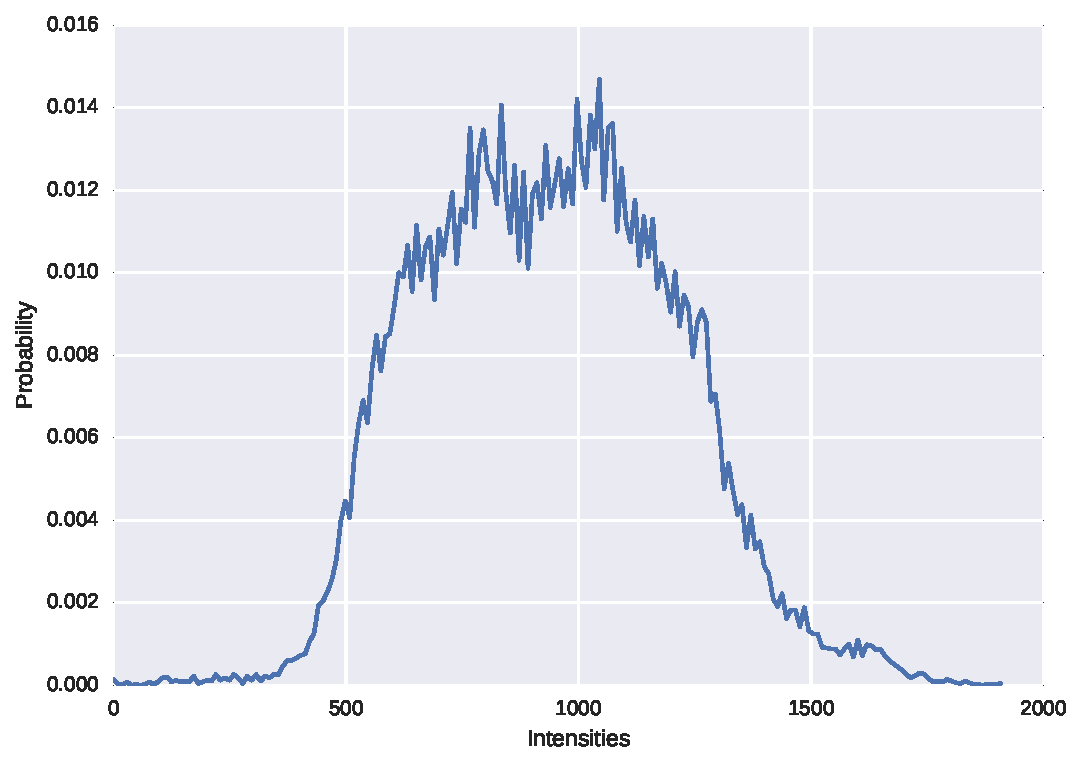
\includegraphics[width=.3\textwidth]{6_pipeline/figures/adc_pdf.pdf}}
  \hfill
  \subfigure[]{\label{fig:adcpdf2}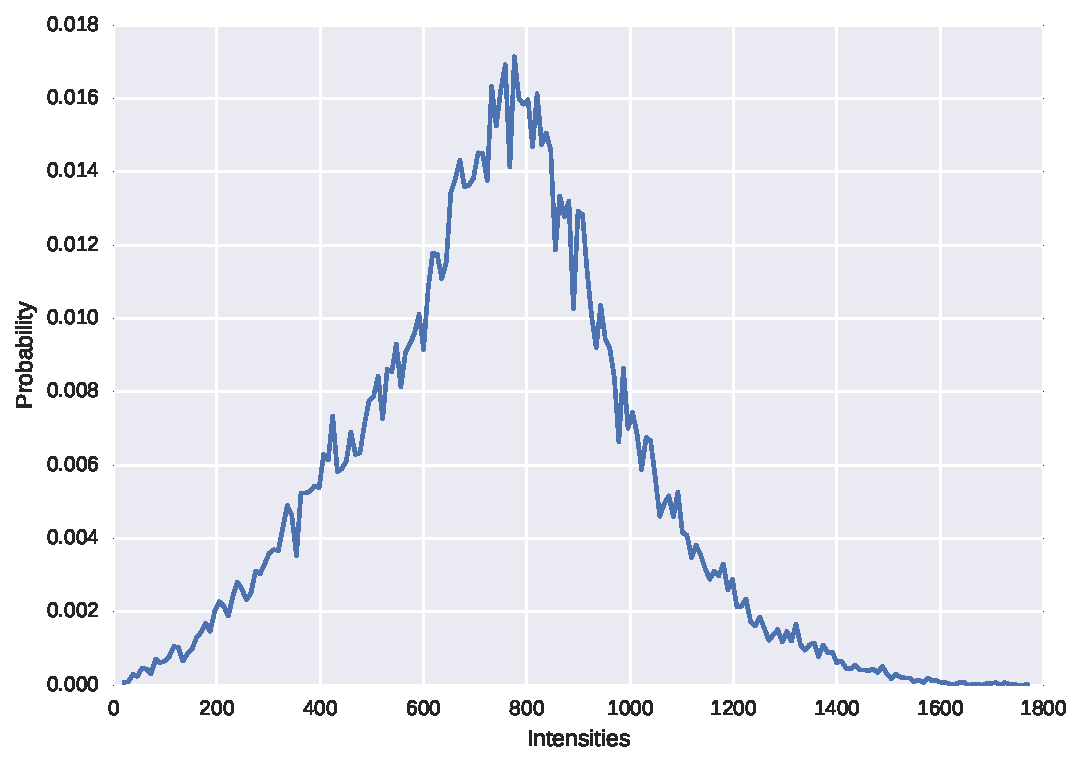
\includegraphics[width=.3\textwidth]{6_pipeline/figures/adc_pdf_2.pdf}}
  \hfill
  \subfigure[]{\label{fig:adcpdf3}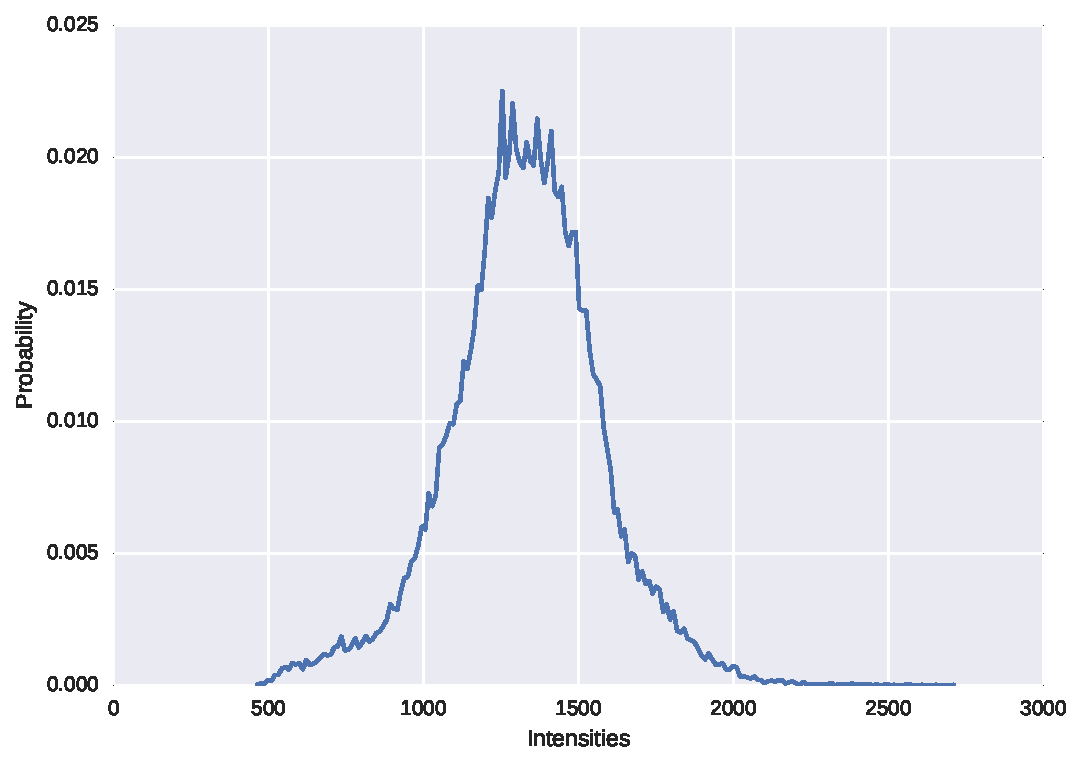
\includegraphics[width=.3\textwidth]{6_pipeline/figures/adc_pdf_3.pdf}}
  \hspace*{\fill}
  \caption[Illustration of the \acs*{pdf} of the \acs*{adc} coefficient within the prostate.]{Illustration of the variability of the \acs*{pdf} of the \acs*{adc} coefficient within the prostate for 3 patients.}
  \label{fig:adcpdf}
\end{figure}


The reader can refer to \acs{sec}\,\ref{subsec:chp3img-reg:prepro} to have an extensive overview of the state-of-the-art methods used to pre-process \ac{mpmri} data.
Three types of pre-processing are used for \ac{mri} images: (i) noise filtering, (ii) bias correction, and (iii) standardization/normalization.
Our dataset is based on \SI{3}{\tesla} images without endorectal coil and therefore, the two first types of correction have not been considered as necessary.
Normalization is, however, a crucial step to reduce the inter-patient variations which allow to improve the learning during the classification stage.
\Ac{chp}~\ref{chap:5} presented 2 normalization methods to pre-process \ac{t2w}-\ac{mri} and \ac{dce}-\ac{mri}, respectively.
Therefore, we used these methods to standardize these images.
Regarding the \ac{adc} map normalization, the \ac{pdf} within the prostate does not follow a known distribution as depicted in \acs{fig}\,\ref{fig:adcpdf}.
Thus, one cannot use a parametric model to normalize these images and a non-parametric piecewise-linear normalization~\cite{Nyul2000} is the best option for this case.

\subsection{Segmentation and registration}\label{subsec:chp6:method:Seg-Reg}

For this study, no segmentation method has been developed and the manual segmentation given by our radiologist has been used.
The prostate is suffering, however, from a misalignment between the different \ac{mri} modalities.
Therefore, three registrations have been developed to: (i) the patient motion during the \ac{dce}-\ac{mri} acquisition, (ii) the patient motion between the \ac{t2w}-\ac{mri} and the \ac{dce}-\ac{mri} acquisitions, and (iii) the patient motion between the \ac{t2w}-\ac{mri} and the \ac{adc} map acquisition.
All registrations are implemented in C++ using \ac{itk}.

The \ac{dce}-\ac{mri} acquisition being dynamic, some intra-patient might occur during the acquisition.
For each serie of this dynamic acquisition, each 3D volume is registered to the first volume acquired, to remove the residual motion.
The appearance in the \ac{dce}-\ac{mri} images, however, varies due to the presence or not of the contrast media.
Therefore, the metric chosen to be minimized is the \ac{mi} and the geometric transform has been set to a rigid transform.
The optimization is performed using a regular step gradient descent.

Once the intra-patient motions corrected, a registration to correct the alignment between the \ac{t2w}-\ac{mri} and the \ac{dce}-\ac{mri} acquisitions is performed.
For that matter, the prostate has been segmented in both modalities --- \ac{t2w}-\ac{mri} and \ac{dce}-\ac{mri} --- to create 2 binary masks.
Therefore, these 3D binary masks are directly registered using the \ac{mse} metric.
Unlike the previous registration, we use a more complex geometric transform by successively finding a rigid transformation, a coarse elastic transformation, and a fine elastic transformation.
B-splines transformation is used as the elastic transform.
These successive transformation allow to get a good initialization for the next transformation.
The transformation is inferred by minimizing the cost function using a regular step gradient descent.

The \ac{t2w}-\ac{mri} and \ac{adc} map acquisitions are identically registered than the the \ac{t2w}-\ac{mri} and the \ac{dce}-\ac{mri} modalities.
Additionally, the \ac{cap}, \ac{pz}, and \ac{cg} are segmented on the \ac{t2w}-\ac{mri} and thus the latter modality is used as the reference modality.

\subsection{Feature detection}\label{subsec:chp6:method:fea-det}
As presented in Sect.~\ref{subsec:chp3:img-clas:CADX-fea-dec}, variety of features have been extracted depending on each modality.
In this work we extract image, \ac{dce}, and \ac{mrsi}-based features from \ac{t2w}-\ac{mri} and \ac{adc}-\ac{mri} images, \ac{dce}-\ac{mri}, and \ac{mrsi}-signals respectively.

Voxel-wise texture, edge, and position-based 3-dimensional features are detected as image-based features.
Laplacian, Prewitt, Sobel, Kirsch operators as well as {\color{red} shaar} and Gabor filter bank are detected as edge-based features.
These features were extensively discussed in Sect.~\ref{subsec:chp3:img-clas:CADX-fea-dec}.
\ac{dct}, \ac{glcm} and \ac{lbp} features are detected as part of texture-based features.

All the \ac{dce}-features presented in Sect.~\ref{subsubsec:chp3:img-clas:CADX-fea-dec:DCE-fea} are extracted from \ac{dce}-\ac{mri} modality.
Whole-spectra, semi-quantitative and quantitative features were explained in details in Chapter.~\ref{chap:5}, Sect.~\ref{subsubsec:chp5:DCE-norm:stateart}.

\ac{mrsi}-based features were previously explained in Sect.~\ref{subsubsec:chp3:img-clas:CADX-fea-dec:MRSI-fea}. 
Whole sepctra and quantification features are extracted from \ac{mrsi}-modality.
  
\subsection{Feature balancing}\label{subsec:chp6:method:fea-bal}
Data imbalanced is a common problem while classifiying medical data.
Considering a binary classification problem, there is always a class (often the class indicating cancer, or disease patients) that have smallest number of samples (i.e, minority class) in comparison to the other class (i.e, majority class).
The problem of data balancing corresponds to equalize the number of samples of both the minority and majority classes.
This task can be achieved in either data or feature space while performing over-sampling of minority samples or under-sampling of majority samples.
In this section we compare different under and over-sampling techniques applied in feature space.

\subsubsection{\Acl*{us1}}
Techniques that reduce the number of samples of the majority class to be equal to the number of samples of minority class are referred as \ac{us1} techniques.
%Considering the problem of imbalanced, \ac{us} is performed such that the number of samples of the majority class is reduced to be equal to the number of samples of the minority class.
The following methods are considered to perform such balancing.

\begin{description}
  \item[\Ac{rus}] is performed by randomly selecting without replacement a subset of samples from the majority class such that the number of samples is then equal in both minority and majority classes.
  \item[\Ac{nm}] offers three different methods to under-sample the majority class~\cite{mani2003knn}.
In \ac{nm1}, samples from the majority class are selected such that for each sample, the average distance to the $k$ \ac{nn} samples from the minority class is minimum.
\ac{nm2} diverges from \ac{nm1} by considering the $k$ farthest neighbours samples from the minority class.
In \ac{nm3}, a subset $M$ containing samples from the majority class is generated by finding the $m$ \ac{nn} from each sample of the minority class.
Then, samples from the subset $M$ are selected such that for each sample, the average distance to the $k$ \ac{nn} samples from the minority class is maximum.
In our experiment, $k$ and $m$ are fixed to 3.
\item[\Ac{iht}]~\cite{smith2014instance} undersamples the samples which have a high hardness threshold.
Hardness indicates the likelihood of missclassification rate for each samples.
The notation of instance hardness are drawn through the decomposition of $p(h \vert t)$ using Bayes' theorem, where $h$ represent the mapping function used to mapp input features to their corresponding labels and $t$ represents the training set.
\begin{equation}
  IH_h(\langle x_{i}, y_{i}\rangle) = 1 - p(y_i \vert x_i, h).\
\label{eq:iht}
\end{equation}
The undersampling is performed by keeping the most probable samples (i.e, filtering the samples with high hardness value) through \ac{kcv} training sets while considering specific threshold for filtering.
%% The hardness of an instance is depedent on the instances in the training data and the algorithm used to produced h (h is a function mapping input features to their corresponding label , i.e, the classifier, or base learner function).

 
\end{description}

\subsubsection{\Acl*{os}}
Contratry to \ac{us1} techniques, the data balancing can be performed by \ac{os} in which the new samples belonging to the minority class are generated aiming at equalizing the number of samples in both classes.
The following methods are compared for \ac{os} techniques.
\begin{description}
\item[\Ac{ros}] is performed by randomly replicating the samples of the minority class such that the number of samples is equal in both minority and majority classes.
\item[\Ac{smote}] is a method to generate synthetic samples in the feature space~\cite{chawla2002smote}.
Let define $x_i$ as a sample belonging to the minority class.
Let define $x_{nn}$ as a randomly selected sample from the $k$ \ac{nn} of $x_i$, with $k$ set to 3.
Therefore, a new sample $x_j$ is generated such that $x_j = x_i + \sigma \left( x_{nn} - x_i \right)$, where $\sigma$ is a random number in the interval $\left[0,1\right]$.
\item[\Ac{smoteb1}]~\cite{han2005borderline} over samples the minority samples similar to \ac{smote}.
However, instead of usig all the minority samples, it focuses on the borderline samples of minority class.
Borderline samples simply indicate the samples that are closer to the other class.
In this method first the borderline samples of minority class are detected.
The sample, $x_{i}$ belongs to borderline samples if more than half of its $k$ \ac{nn} samples belong to majority class.
Synthetic data is then created based on \ac{smote} method for borderline samples and selection of their $s$ \ac{nn} from the minority class.
 
\item[\Ac{smoteb2}]~\cite{han2005borderline} performs similar to \ac{smoteb1}.
However, instead of generating synthetic samples from borderline samples and their $s$ \ac{nn} from the minority class, it also generate samples based on their \ac{nn} of majority samples.
Synthetic samples created based on majority samples are placed closer to samples of minority class.
\end{description}

\subsection{Feature selection and extraction}\label{subsec:chp6:method:fea-sel}
Different feature selection and extraction methods were presented in Sect.~\ref{subsec:chp3:img-clas:CADX-fea-ext}.
Among those \ac{pca} is used as feature extraction on  \ac{mrsi} and \ac{dce}-based features.
In addition to \ac{pca}, sparse-\ac{pca} and \ac{ica} are also used to extract distinct features from \ac{mrsi} and \ac{dce}-based features.

Similar to \ac{pca}, \ac{ica}~\cite{comon1994independent} is looking for independent components of the datat.
However, it does not require orthogonolaity of the space and does not assume Gaussian distribution for each independent source.
Therefore, opposit to \ac{pca} it can recover uniquely the signals themselve rather than  linear subspace in which the signals lie \cite{murphy2012machine}.

Sparse-\ac{pca}~\cite{zou2006sparse} is another approach for feaure extraction and dimension reduction.
Similar to \ac{pca}, this apprcoach project the data into linear combination of input data.
However, instaed of using original data, it uses the sparse representation of the data, and therefore projects them as linear combination of few input components rather than all of them.
Refereing to Eq.~\eqref{eq:eigpca}, the objective of sparse-\ac{pca} is formulated as maximizing the variance while maintinaing the sparse constraint:

\begin{eqnarray}
 && \argmax \quad   \mathbf{v}^{-1} \Sigma \mathbf{v}\ , \label{eq:sparsepca}\\ 
 && \text{subject to }  \Vert \mathbf{v} \Vert_{2} = 1\ , \nonumber \\
 && \Vert \mathbf{v} \Vert_{0} \leq k\ . \nonumber
\end{eqnarray}
\noindent where $k$ indicates that number of non-zero elements in $\mathbf{v}$.

ANOVA F-test and \ac{rf} are used as feature selection approaches for image-based features.
ANOVA F-test can assess the superiority or inferiority of the features 
ANOVA F-test evaluates the potential of one feature at a time to predict the target label by measuring between group variability over within group variability.
This test finds which features on average are superior of inferior to others versus the null hypothesis.
%% \begin{equation}
%% F = \frac{}{}
%% \label{eq:Ftest}
%% \end{equation} 


\subsection{Classification}\label{subsec:chp6:method:clas}
Variety of classifiers were explained in Sect.~\ref{subsec:chp3:img-clas:CADX-clas}. 
Among those \ac{rf} is used as ensemble approach while classifying inidiviual modalities, where as a meta classifier using stacking of \ac{rf} is used for combination of different modalities.

Staking~\cite{wolpert1992stacked} is a way to create a meta classifier using different base learners.
This method uses the prediction of different base learners as input for a meta leaner and combines them into a final decision.
Each base learner is trained on the training set and its prediction on the validation set is fet to the meta learner.
The test sample, in a similar way is first classified by the base learners and their prediction is passed through the meta learner in order to achieve the final decision.

 


\section{Experiments and results}\label{sec:chp6:exp-res}
To evaluate different aspects of the proposed \ac{cad} system, we proposed variety of experiments with respect to individual modalities and their combination. 
Table~\ref{tab:exp-summary} represents the summary of the experiments. 
These experiments and the results obtained are discussed in details in the reminder of this section. 
Pre-processing, segmentation and registration of each modalities are common steps across all the designed experiments.

\subsection{Experiment-1: Assessment of inidivual modalities}\label{subec:chp6:exp-res:Ex1} 
The main goal of this experiment is to eavluate the potential of each inividual modality and their corresponding features. 
Different features as presented in Sect.~\ref{subsec:chp6:method:fea-det} are extracted for different modalities. 
For all the modalities, the extracted features without any extraction or selection process are used to train a \ac{rf} classifier, using a \ac{lopo}. 
These experiments are performed using {\color{red} which dataset}.
The results are presented in terms of \ac{roc} analysis and averaged \ac{auc} over \ac{lopo}.
Figure~\ref{fig:res-Ex1} illustrate the obtained results.

\begin{figure}
  \hspace*{\fill}
  \subfigure[Performance of different pharmacokinetic paramters on \ac{dce}-\ac{mri}]{\label{fig:}\includegraphics[width=.49\textwidth]{5_normalization/figures/DCE-normalization/normalized_methods_0.pdf}}
  \hfill
  \subfigure[Performance of whole \ac{dce}-\ac{mri} signal]{\label{fig:}\includegraphics[width=.49\textwidth]{5_normalization/figures/DCE-normalization/full_signal_0.pdf}}
  \hspace*{\fill} \\
  \hspace*{\fill}
  \subfigure[Performance of image-based features for \ac{t2w} and \ac{adc}-\ac{mri}]{\label{fig:}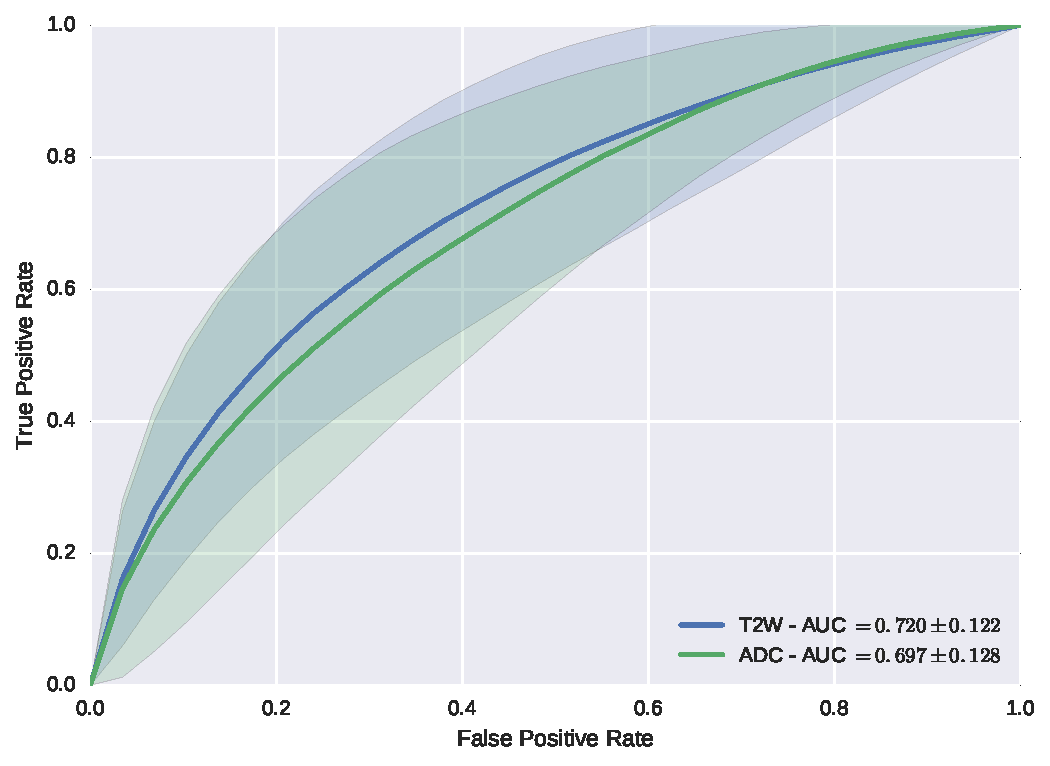
\includegraphics[width=.49\textwidth]{6_pipeline/figures/exp-1/t2w_adc.pdf}}
  \hfill
  \subfigure[Performance of whole spectra using \ac{mrsi} signal]{\label{fig:}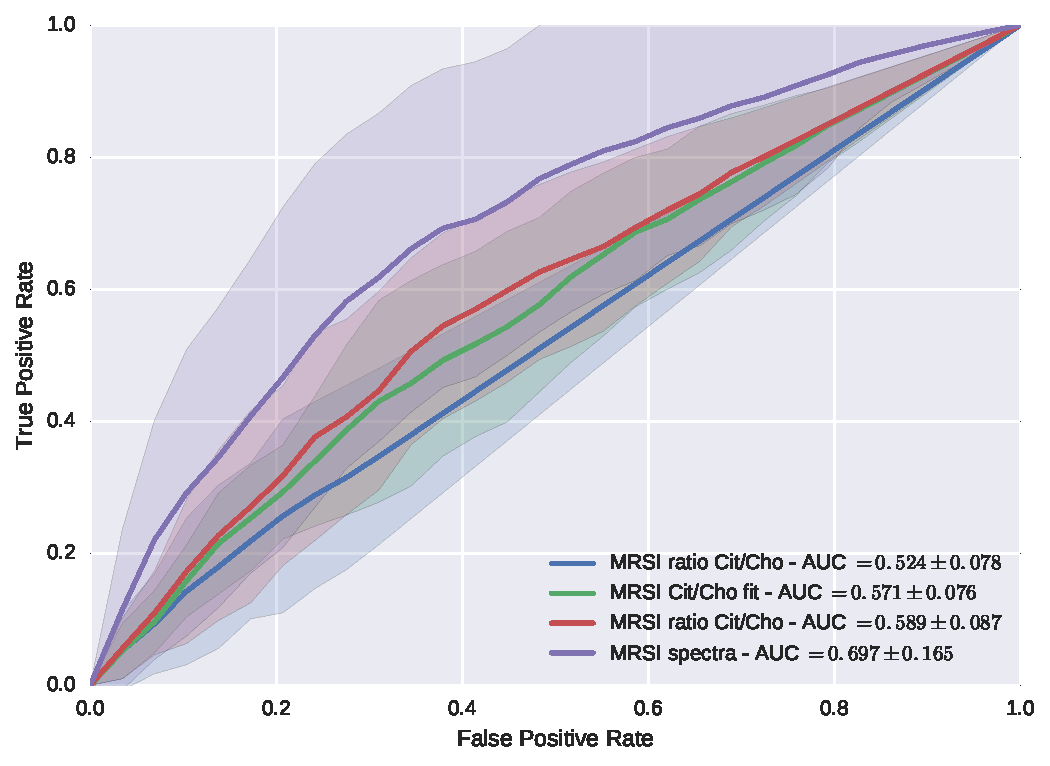
\includegraphics[width=.49\textwidth]{6_pipeline/figures/exp-1/mrsi_all.pdf}}
  \hspace*{\fill}
  \caption[Results obtained from experiment-1]{Results obtained from experiment-1: assessment of inividual modalities}
  \label{fig:res-Ex1}
\end{figure}


\subsection{Experiment-2: Coarse combination} \label{subsec:chp6:exp-res:Ex2}
The objective of this experiment is to evaluate the combination of all the modalities.
To this extent, three different approaches are considered: (i) feature aggregation, (ii) statcking using \ac{adb}, (iii) stacking using \ac{gb}. 
In the first approach, feature aggregation, the features extracted from each modalities (\ac{t2w}, \ac{adc}, normalized-whole-\ac{dce} and normalized-whole-\ac{mrsi}, as concluded in experiment-1) are concatenated together and used with a \ac{rf} classifier and \ac{lopo}. 
In the second and third approach since stacking is used the training set is divided into training and validation set.
Therefore, first a \ac{rf} classifier is trained for each modality using the their corresponding training set and then using a validation set their prediction is fed as a training to a meta learner.
\Ac{adb} and \ac{gb} are used as a meta learner for the second and third approach, respectively. 
Figure~\ref{fig:flow-Ex2} shows the framework of the first and second/third approach. 

The obtained results of this experiment are shown in Fig.~\ref{fig:res-Exp2}.
\begin{figure}
  \centering
  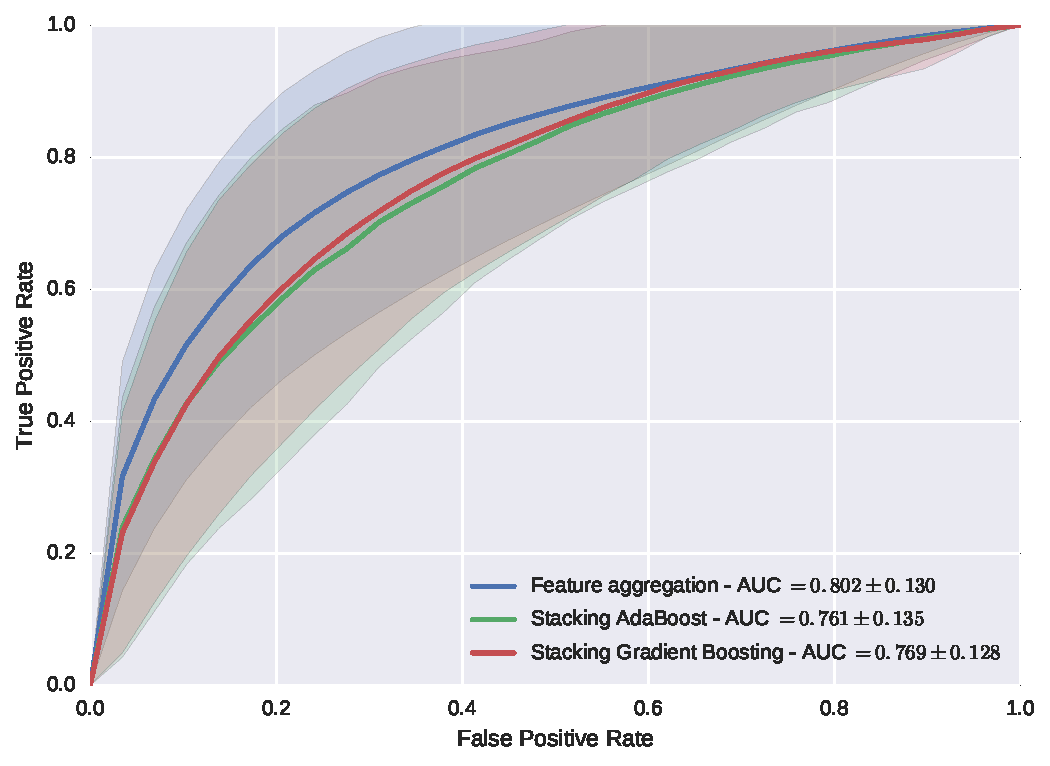
\includegraphics[width=0.7\linewidth]{6_pipeline/figures/exp-2/comb_all.pdf}
  \caption[Results obtained from experiment-2]{Results obtained from experiment-2: Coarse combination of different modaliies.}
  \label{fig:res-Exp2}
\end{figure}

\subsection{Experiment-3: Fine tuning}\label{subsec:chp6:exp-res:Ex3}
In the previous experiments (1 \& 2) the original features were used, without any adjustment or tunning. 
In this section, as we call it fine tuning, first we evaluate the performance and benefits of having a balance set, then we eavaluate different feature selection and extraction techniques.
The main aim of this experiment is to find the best balancing technique and feature selection approach suited for each modality. 
Therefore, simiar to experiment-1, only the performance of individual modalities are comapered. 

The \ac{us1} and \ac{os} techniques used to balance our training set were explained in Sect.~\ref{subsec:chp6:method:fea-bal}.
Figure~\ref{fig:res-Ex3-bal} shows the comparison of these techniques on each modality. 
\begin{figure}
  \hspace*{\fill}
  \subfigure[\ac{t2w}-\ac{mri}]{\label{fig:ex3:T2W}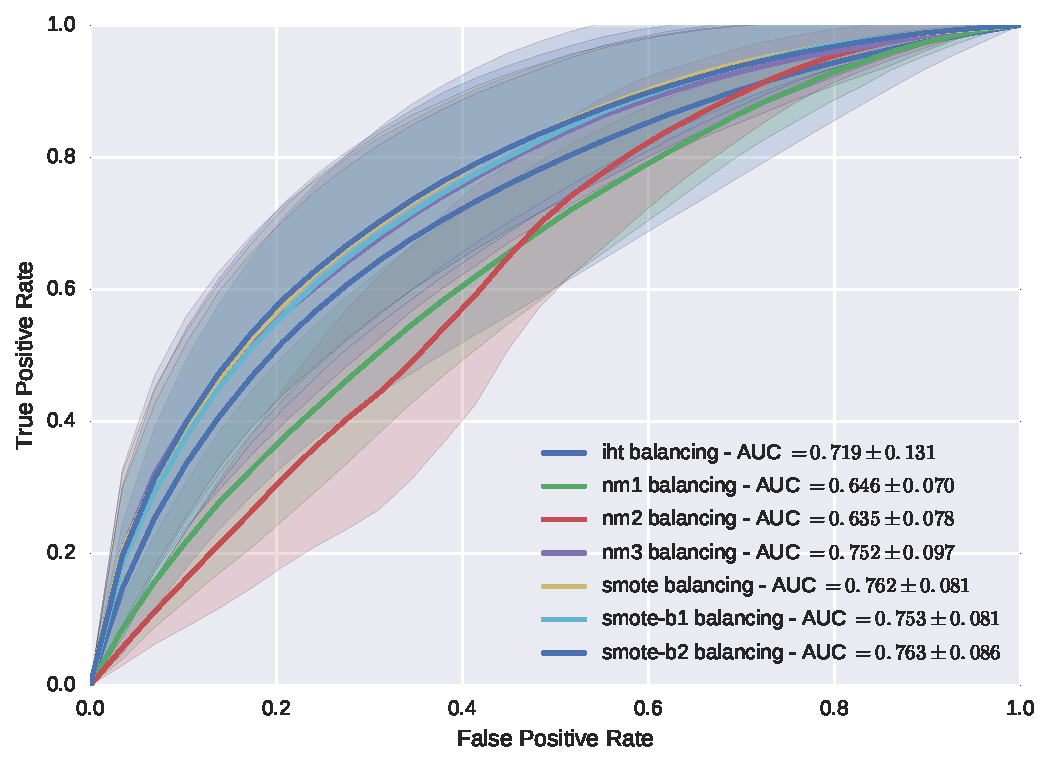
\includegraphics[width=.49\textwidth]{6_pipeline/figures/exp-3/t2w.pdf}}
  \hfill
  \subfigure[\ac{adc}-\ac{mri}]{\label{fig:ex3:ADC}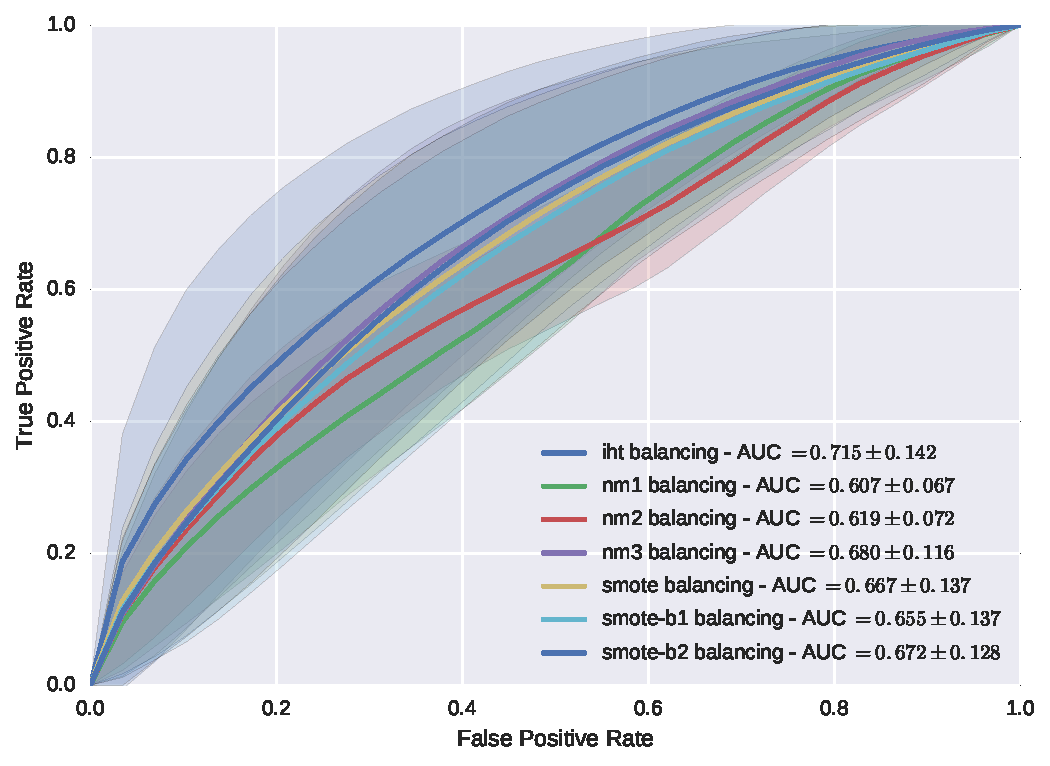
\includegraphics[width=.49\textwidth]{6_pipeline/figures/exp-3/adc.pdf}}
  \hspace*{\fill} \\
  \hspace*{\fill}
  \subfigure[\ac{dce}-\ac{mri}]{\label{fig:ex3-DCE}\includegraphics[width=.49\textwidth]{6_pipeline/figures/exp-3/dce.pdf}}
  \hfill
  \subfigure[\ac{mrsi}-\ac{mri}]{\label{fig:ex3-MRSI}\includegraphics[width=.49\textwidth]{6_pipeline/figures/exp-3/mrsi.pdf}}
  \hspace*{\fill}
  \caption[Results obtained from experiment-3: balancing techniques.]{Results obtained from experiment-3: comparison of differnet balancing techniques on individual modalities}
  \label{fig:res-Ex3-bal}
\end{figure}

\subsection{Experiment-4: Fine combination}\label{subsec:chp6:exp-res:Ex4}
This experiments evaluates the combination of all the modalities after applying fine tunning and adjusting the feature space. 
Two different approaches are compared: (i) Feature aggregation and (ii) stacking using \ac{gb}. 
The second approach of experiment-2 was ignored, since as previously concluded, \ac{gb} had a slightly better performance than \ac{adb}.

\begin{figure}
  \centering
  \includegraphics[width=0.7\linewidth]{6_pipeline/figures/exp-5/combine_all.pdf}
  \caption[Results obtained from experiment-4]{Results obtained from experiment-4: Fine combination of different modalities.}
  \label{fig:res-Ex4}
\end{figure}


\section{Discussion}\label{sec:chp6:discussion}

%%% Local Variables: 
%%% mode: latex
%%% TeX-master: "../thesis"
%%% End: 


%% \section{Discussion}\label{sec:chp3:dis}


\subsection{Results reported}\label{subsec:chp3:dis:res}

As discussed previously in \ac{sec}\,\ref{subsec:chp3:img-clas:eval-mea}, different metrics have been used to report results.
A comparison of the different methods reviewed is given depending on the metric used in field of research and also the type of \ac{mri} scanner used, i.e. \SI{1.5}{\tesla} or \SI{3}{\tesla}.
For each field, the \textit{best classification performance} obtained in each study have been reported in these figures.
The results in terms of \ac{auc}-\ac{roc} are depicted in \acs{fig}\,\ref{fig:auc}.
The results vary from \SIrange{71}{97}{\percent} for some experiments with a \SI{1.5}{\tesla} \ac{mri} scanner and from \SIrange{77}{95}{\percent} with a \SI{3}{\tesla} \ac{mri} scanner. 

The results in regard of sensitivity and specificity are reported in \acs{fig}\,\ref{fig:sensspec}.
In the case that the data have been collected with a \SI{1.5}{\tesla} \ac{mri} scanner, the sensitivity ranges from \SIrange{74}{100}{\percent} and the specificity from \SIrange{43}{93}{\percent}.
For the experiments carried out with a \SI{3}{\tesla} \ac{mri} scanner, the sensitivity varies from \SIrange{60}{99}{\percent} and the specificity from \SIrange{66}{100}{\percent}.
Four studies also use \ac{froc} analysis to report their results and are reported in \ac{fig}\,\ref{fig:froc}.

\begin{figure}
  \centering
  \includegraphics[width=.8\linewidth]{3_review/figures/results/froc.eps}
  \caption{Comparison in terms of \acs*{froc} of the methods using data from \SI{3}{\tesla} \acs*{mri} scanner.}
  \label{fig:froc}
\end{figure}

\input{3_review/fig-res-auc.tex}
\input{3_review/fig-res-SESP.tex}

\subsection{Comparison}\label{subsec:chp3:dis:com}

We would like to stress the following findings drawn during the review of the different studies:

\begin{enumerate}
\item Quantitatively, it is difficult to make a fair comparison between the different studies reviewed.
Different factors come into play to elucidate this fact.
Mainly a lack of standardization has to be pointed out in regard to experimental evaluation:
(i) different datasets are used during the evaluation of the frameworks developed hindering an inter-study comparison.
The same conclusion has been recently drawn by~\cite{Litjens2014} supporting this argument;
(ii) the experimental results are not reported with a common metric which leads to the inability to compare the different studies.

\item \label{here} However, multiple studies reported some performance improvements using \ac{mpmri} techniques instead of mono-parametric imaging techniques.
Considering only the most recent studies proposing \ac{cade}-\ac{cadx} frameworks, the following results can be highlighted.
\citeauthor{Viswanath2011} obtained an \ac{auc} of \SI{77}{\percent} using an ensemble learning approach combining the features from the three \ac{mri} modalities --- i.e., \ac{t2w}-\ac{mri}, \ac{dce}--\ac{mri}, and \ac{dw}-\ac{mri}, while the results obtained as standalone modality range from \SIrange{62}{65}{\percent}~\cite{Viswanath2011}. 
\citeauthor{Tiwari2013} drawn similar conclusions by using \ac{t2w}-\ac{mri} and \ac{mrsi} modalities as both in standalone and multi-parametric frameworks with an improved \ac{auc} ranging from \SI{57}{\percent}-\SIrange{76}{85}{\percent}~\cite{Tiwari2013}.
The most recent work of \citeauthor{Litjens2014} obtained an improved \ac{auc} metric from \SI{71}{\percent}-\SI{76}{\percent} considering each modality separately --- i.e., \ac{t2w}-\ac{mri}, \ac{dce}-\ac{mri}, and \ac{dw}-\ac{mri} --- to \SI{89}{\percent} in their \ac{mpmri} framework.

\item The studies comparing particular combination of more than a single modality give rise to the same fact~\cite{Ozer2010,Litjens2011,Liu2013,Litjens2014}: using 3 modalities lead to better performances than using any combination of 2 modalities. 

\item Unlike the previous remark~\ref{here}, no straightforward conclusions can be given regarding the classification performance using each modality in a standalone framework.
The modality being processed by different methods, it does not allow us to conclude if a modality by itself is more suited than another.
However, we are able to distinguish some interesting trends which deserve the attention of the community.
\citeauthor{Tiwari2013} in~\cite{Tiwari2009a,Tiwari2012,Tiwari2013} observed that \ac{mrsi} is a more suitable modality than \ac{t2w} to highlight \ac{cap}.
Moreover, \ac{adc} maps have shown a better discriminative power than \ac{t2w} as well~\cite{Langer2009,Viswanath2011,Peng2013}.
Lately, \citeauthor{Litjens2014} observed that \ac{dw}-\ac{mri} modality is more suitable than both \ac{dce}-\ac{mri} and \ac{t2w}-\ac{mri} to distinguish \ac{cap} in their \ac{cadx} system~\cite{Litjens2014}. 
Recently, \citeauthor{rampun2016computerb} showed, however, some promising results using \ac{t2w}-\ac{mri} only in conjunction with textons and \ac{bow}; this study should be transposed to other \ac{mri} modalities~\cite{rampun2016computerb}.

\item Furthermore, \ac{mpmri} has attracted the attention of both radiologists and computer vision researchers.
Indeed, pioneer research groups included new modalities over years when at the same time, new research groups directly introduced \ac{mpmri} \ac{cad} systems.
These facts lead us to think that \ac{cap} researches will benefit from \ac{mpmri} techniques.

\item When focusing on the different modalities used, it can be pointed out that only \citeauthor{trigui2017automatic} reported the use of all modalities in a single framework by incorporating the \ac{mrsi} modality~\cite{trigui2016classification,trigui2017automatic}.
Although the results reported are promising, the detection has been performed at \ac{mrsi} scale and further investigations need to be carried out.
Nevertheless, \ac{mrsi} has shown some overall good classification performance at the price of a lower resolution as well as an increased acquisition time.
Moreover, \ac{mrsi} analysis is more complex in comparison with the other modalities.
To our mind, \ac{mrsi} could contribute in a \ac{mpmri} framework and should be fused with the other modalities.

\item Lately, 3 studies focused on developing a region-based classification in which \ac{pz} and \ac{cg} will be analyzed separately~\cite{Viswanath2012,Litjens2012,Litjens2014}.
The promising obtained results indicate that this strategy should be further investigated.

\item Recent studies are using quantitative features in addition to \ac{si}.
It seems that these quantitative features provide uncorrelated information with respect to \ac{si} features and should lead to better classification performance when combined all together. 

\item Regarding the methods used in the ``image regularization'' --- i.e., pre-processing, segmentation, and registration --- it is particularly difficult to distinguish the benefit of a method over another since none of the studies focus on making comparison of these processing stages.
The focus is usually entirely based on the ``image classification'' framework where different methods are directly compared.
Note that the performance of a classifier is highly linked with the features vector extracted from particular data.
Hence, one can not conclude that a machine learning method is more appropriate than another, but we can identify a trend in which \ac{svm} as well as ensemble learning classifiers --- i.e., AdaBoost, GentleBoost, and \ac{rf} --- seem to perform better than neural network, \ac{lda}, or Naive Bayes.

\item We would like to draw the attention of the reader on the feature extraction/selection stage.
This processing could reduce the complexity and also allow to find a better feature space for classification.
However, few studies are performing such approaches.
\citeauthor{Niaf2012}, \citeauthor{khalvati2015automated}, \citeauthor{chung2015prostate}, and \citeauthor{rampun2016computer} are successfully applying a scheme to reduce the number of dimensions by selecting the most discriminative features~\cite{Niaf2011,Niaf2012,khalvati2015automated,chung2015prostate,rampun2016computer,rampun2015computer}.
It allows them to obtain improved performances compared with a classification performed with their initial feature vector.
Another group of studies also applied different feature extraction methods~\cite{Viswanath2008a,Viswanath2008,Viswanath2012,Tiwari2007,Tiwari2008,Tiwari2009,Tiwari2010,Tiwari2012,Tiwari2013,lehaire2014computer,rampun2016computerb,rampun2015classifying}.
In these specific cases, no comparison is performed against the original data.
\end{enumerate}

\section{Conclusion}\label{subsec:chp3:dis:gen-dis}

This review leads to some general discussions which could direct to future avenues for research.
As previously mentioned, no open \ac{mpmri} is currently available.
This fact leads to an impossibility to fairly compare the different algorithms designed over years.
Also, the availability of a full \ac{mpmri} dataset, could lead to the development of algorithms which use all the different modalities currently available.
Recalling \acs{tab}~\ref{tab:sumpap}, it can be noted that a single research work provides a solution using at the same time the 4 different modalities.
Also, all the algorithms are focused on one type of scanner only, either \SI{1.5}{\tesla} and \SI{3}{\tesla}.
A dataset including both these types of imaging could allow development of more generic algorithms.

Analyzing the different stages of the \ac{cad} work-flow, it is seen that the current \ac{cad} systems do not include all the pre-processing steps.
It could be interesting to evaluate the improvement using these pre-processing steps on the final results.
Regarding segmentation and registration of the prostate, \ac{cad} systems could greatly benefit from specific research in these areas which could lead to a better automation of those systems.
%Moreover, other segmentation and registration methods does not currently used in \ac{cad} systems could also obtain better results.

% Regarding the classification framework, it seems that the current well-known pattern recognition methods have been widely studied.
% However, more investigations should be carried out regarding the feature detection stage.
% Lately, histogram-based features have shown good capabilities in the field of computer vision and could be further investigated.
% Only one study by~\cite{Liu2013} used some of these features.

Additionally, no research focus on the problem of imbalanced dataset.
While classifying at the voxel-level, the medical dataset are highly imbalanced regarding the frequencies of \ac{cap} against healthy samples.
Imbalanced data substantially compromises the learning process since most of the standard machine learning algorithms expect balanced class distribution or an equal micslassification cost~\cite{he2009learning}.
Therefore, it seems important to investigate this field of pattern recognition to improve the classification performance while developing \ac{cad} systems.

%An important point allowing a fair comparison between methods resides in the fact that no common dataset, nor universal evaluation model, nor metric has been defined by the research community allowing such comparison.
% This review aims to have an impact in that respect by providing a novel publicly available multi-parametric and multi-vendor \ac{mri} dataset (from a 1.5 Tesla General Electric scanner and a 3.0 Tesla Siemens scanner).
% This dataset is available at the following website address: \url{http://visor.udg.edu/dataset}. The dataset is composed of the four modalities discussed in this review with their corresponding ground-truth images. For each scanner type, each subset is composed of twenty patients with cancerous lesions and ten healthy patients, having a total of 60 patients. In addition of the repository activity, this website will aim at providing comparison between algorithms developed by the research community.

Therefore, the main objectives of this thesis are to: (i) collect and make available the first \ac{mpmri} dataset; (ii) design, develop, and investigate a \ac{cad} system taking advantage of all available \ac{mri} modalities; (iii) focus on pre-processing methods to improve the classification performance of \ac{cad} systems; (iv) investigate the problem of imbalanced dataset in the \ac{cad} performance; (v) release source code to allow future benchmarking.
               % discussion of results

\begin{appendices}
\chapter{Conversion from FLASH signal to media concentration}\label{app:signaltoconc}

In this appendix, we show the demonstration used to extract the agent concentration from the \ac{mri} signal.

The signal equation in FLASH sequence~\cite{haase1986flash} is defined as:

\begin{equation}
  s(t) = S_{eq} \sin \alpha \cdot \frac{1 - \exp\left(-TR\left(R_{10} + r_1 c(t)\right)\right)}{1 - \cos \alpha \cdot \exp\left(-TR\left(R_{10} + r_1 c(t)\right)\right)} ,
  \label{eq:app:flash}
\end{equation}

\noindent where $s(t)$ is the \ac{mri} signal, $S_{eq}$ is the maximum signal amplitude of the spoiled gradient at the \ac{te} which is proportional to the \ac{pd}, $\alpha$ is the flip angle, $TR$ is the \acf{tr}, $R_{10}$ is the pre-contrast tissue relaxation time also equal to $\frac{1}{T_{10}}$, $r_1$ is the relaxitivity coefficient of the contrast agent, and $c(t)$ is the media concentration.

Therefore, the pre-contrast signal prior to bolus injection of the media is defined as:

\begin{equation}
  S_0 = S_{eq} \sin \alpha \cdot \frac{1 - \exp\left(-TR \cdot R_{10}\right)}{1 - \cos \alpha \cdot \exp\left(-TR \cdot R_{10}\right)} .
  \label{eq:app:precontrast}
\end{equation}

To simplify the demonstration, let us define:

\begin{align}
  A &= \exp(-TR \cdot R_{10}) , \\
  B &= \exp(-TR \cdot r_1 c(t)) .
\end{align}

Let us define:

\begin{align}
  S^{*} &= \frac{S_0}{S_{eq} \sin \alpha} , \\
  &= \frac{1 - A}{1 - A \cos \alpha} .
\end{align}

Thus,

\begin{align}
  S^{*}\frac{s(t)}{S_0} &= \frac{S_0}{S_{eq}\sin \alpha} \frac{s(t)}{S_0} , \\
  &= \frac{1 - A B}{1 - A B \cos \alpha} .
\end{align}

Now, let us define:

\begin{align}
  \frac{1 - \cos \alpha \cdot S^{*}\frac{s(t)}{S_0}}{1 - S^{*}\frac{s(t)}{S_0}} &= \frac{ 1 - \cos \alpha\left(\frac{1 - A B}{1 - A B \cos \alpha}\right)} {1 - \frac{1 - A B}{1 - A B \cos \alpha}} , \\
  &= \frac{1 - A B \cos \alpha - \cos \alpha(1 - A B)}{1 - A B \cos \alpha - (1 - A B)} , \\
  &= \frac{1 - A B \cos \alpha - \cos \alpha + A B \cos \alpha}{1 - A B \cos \alpha - 1 + A B} , \\
  &= \frac{1 - \cos \alpha}{ A B (1 - \cos \alpha)}, \\
  &= \frac{1}{A B}.
\end{align}

Thus,

\begin{equation}
  -TR \cdot R_{10} -TR \cdot r_1 c(t) = \ln\left( \frac{1 - \cos \alpha \cdot S^{*}\frac{s(t)}{S_0}}{1 - S^{*}\frac{s(t)}{S_0}} \right) .
\end{equation}

Therefore,

\begin{equation}
  c(t) = \frac{1}{TR \cdot r_1} \ln\left( \frac{1 - \cos \alpha \cdot S^{*}\frac{s(t)}{S_0}}{1 - S^{*}\frac{s(t)}{S_0}} \right) - \frac{R_{10}}{r_1} .
\end{equation}


\end{appendices}

%%% Local Variables: 
%%% mode: latex
%%% TeX-master: "../thesis.tex"
%%% End: 
        % description of lab methods




% --------------------------------------------------------------
%:                  BACK MATTER: appendices, refs,..
% --------------------------------------------------------------

% the back matter: appendix and references close the thesis


%: ----------------------- bibliography ------------------------

% The section below defines how references are listed and formatted
% The default below is 2 columns, small font, complete author names.
% Entries are also linked back to the page number in the text and to external URL if provided in the BibTex file.

% PhDbiblio-url2 = names small caps, title bold & hyperlinked, link to page 
%\begin{multicols}{2} % \begin{multicols}{ # columns}[ header text][ space]
%\begin{tiny} % tiny(5) < scriptsize(7) < footnotesize(8) < small (9)

%\bibliographystyle{Latex/Classes/PhDbiblio-url2} % Title is link if provided
\bibliographystyle{abbrvnat} % calls style file plainnat.bst

\renewcommand{\bibname}{References} % changes the header; default: Bibliography

%\bibliography{9_backmatter/references} % adjust this to fit your BibTex file
\bibliography{9_backmatter/literature_review_2}

%\end{tiny}
%\end{multicols}

% --------------------------------------------------------------
% Various bibliography styles exit. Replace above style as desired.

% in-text refs: (1) (1; 2)
% ref list: alphabetical; author(s) in small caps; initials last name; page(s)
%\bibliographystyle{Latex/Classes/PhDbiblio-case} % title forced lower case
%\bibliographystyle{Latex/Classes/PhDbiblio-bold} % title as in bibtex but bold
%\bibliographystyle{Latex/Classes/PhDbiblio-url} % bold + www link if provided

%\bibliographystyle{Latex/Classes/jmb} % calls style file jmb.bst
% in-text refs: author (year) without brackets
% ref list: alphabetical; author(s) in normal font; last name, initials; page(s)

%\bibliographystyle{plainnat} % calls style file plainnat.bst
% in-text refs: author (year) without brackets
% (this works with package natbib)


% --------------------------------------------------------------

% according to Dresden med fac summary has to be at the end
%\include{0_frontmatter/abstract}

%: Declaration of originality
\include{9_backmatter/declaration}



\end{document}
